\chapter{Fejlesztői dokumentáció} % Developer guide
\label{ch:impl}

A tesztek futtatásához (amennyiben nincs egyéb meghatározva) egy asztali számítógépet használtam a következő paraméterekkel:

\begin{table}[h]
\centering
    \begin{tabular}{|l|l|l|}
        \hline
        \textbf{Megnevezés} & \textbf{Modell} & \textbf{Megjegyzés} \\
        \hline
        Alaplap & ASUS Prime X470-PRO & \\
        \hline
        CPU & Ryzen 7 2700X 8c/16t 4.00Ghz & alap órajel \\
        \hline
        RAM & Corsair Vengeance 2x8GB 2400Mhz DDR4 dual channel & \\
        \hline
        GPU & Nvidia Geforce GTX 1070 & alap órajel \\
        \hline
        SSD & Samsung 970 EVO 250GB & NVMe slot \\
        \hline
    \end{tabular}
    \caption{A tesztekhez használt számítógép paraméterei.}
\end{table}


% ------------------- OpenCL Basics
\section{Az OpenCL}



% Basics
\subsection{Alapok}


\begin{definition}
Heterogén rendszer: több processzor együttműködésén alapuló számítógépes rendszer.
\end{definition}

\begin{definition}
uint: egy 32 biten tárolt előjel nélküli (csak pozitív) egész szám, amelyen minden műveletet $mod \; 2^{32}$ értelmezünk.
\end{definition}


Az OpenCL egy nyílt forráskódú, cross-platform keretrendszer olyan homogén számítógépes környezetekhez, ahol a CPU és GPU vagy egyéb processzorok és ezek szálai párhuzamos együttműködésére van szükség. \cite{munshi2011opencl}.


\begin{definition}
Hoszt (host): Több processzoros rendszerek esetén azon eszköz, amely a többi irányításáért felel.
\end{definition}

\begin{definition}
Eszköz (device): Több processzoros rendszerek esetén azon eszköz, amely a hoszttól kapott feladatokat ellátja.
\end{definition}


A keretrendszer egy saját programozási nyelvvel rendelkezik, mely a C nyelvből fejlődött ki. Úgynevezett kerneleket tudunk írni, amelyekez az eszközökön tudunk futtatni. A projekt során a C++ API-t fogom alkalmazni, azonban sok nyelvhez elérhető hasonló könyvtár.

Az OpenCL keretrendszer inicializálásakor megadható hogy melyik eszközöket használjuk, illetve milyen szerepet fognak ezek betölteni. Szerepe alapján a hardvereket hoszt és eszköz kategóriákra bonthatjuk. Emellett fontos különbség az adott hardverek platform-ja. Minden platform különböző implementációját futtatja a az OpenCL keretrendszernek (pl.: Intel, AMD, Nvidia).

A program fordításának idejében nem ismerjük a jövőbeli felhasználó számítógépének pontos paramétereit, holott ez elengedhetetlen információ a fordító számára. Erre két megoldás közül tudunk választani:


\begin{enumerate}
  \item A kódot minden napjainkban használt eszközre optimalizálva lefordítjuk, illetve a későbbiekben amennyiben ez változik, új verziókat készítünk.
  \item Nem fordítjuk azonnal az eszközre szánt kernel kódot, ehelyett azt eltároljuk a program számára elérhető helyen, majd amikor a felhasználó először futtatja a programot, lefordítjuk a kernelt.
\end{enumerate}


Látszik hogy az első megoldás szinte kivitelezhetetlen, hiszen naprakészen tartani több ezer vagy akár tízezer konfigurációt lényegesen nagyobb költséggel jár, mint a felhasználó számára az első alkarommal várni akár kevesebb mint egy másodpercet hogy leforduljon a kód. A második megoldás hátránya azonban, hogy nem tudjuk elrejteni a kernel kódunkat és az könnyen másolható lesz. Ezzel szemben a kód futásidpőben szerkeszthető marad, amely tulajdonságát ki fogom használni a program során.


\lstset{caption={Tetszőleges méretű vektor összeadása OpenCL kernellel (forrás: Elte IK Computer Graphics GPGPU)}, label=src:cpp}
\begin{lstlisting}[language={C++}]
kernel void add(global const int* A,
                global const int* B,
                global int* C)
{ 
    int i = get_global_id(0); //Global ID in dimension 1 (0)
    C[i] = A[i] + B[i]; 
}
\end{lstlisting}



% Optimization
\subsection{Optimalizálás}

A szakdolgozat jelentős részét képzi az eszköz oldali parallel kód futásának optimalizálása. Ezen optimalizálás a lefordított kód elemzésével történhet legeffektívebben. Ehhez az AMD APP Kernel Anayzer-t használtam. Ez az eszköz a lefordított programkód utasításait visszafejti assebmly nyelvre. Az assembly kód betekintést adhat az esetleges optimálatlan kódrészekbe. 

Videókártyák esetén egy potenciális \SI{50}{\percent} lassítást jelenthet az elágazások használata. A futó szálak egyszerre egy parancsot képesek elvégezni, így aztán amíg bizonyos szálak egy elágazás hosszabb igaz oldalával dolgoznak, addig a többinek várni kell azokra még akkor is, ha gyorsabban végeztek a második felével. Ez alapján mindig elkerülöm a balanszolatlan hosszúságú elágazásokat, de igyekszem őket ahol csak lehetséges nélkülözni.

Szintén nagyobb teljesítményromálssal járhat a ciklusok használata. Egy ciklus minden lépése egy memóriacím növelésével, illetve egy elágazással jár. Emellett a cikluson belül felhasznált iterátor változót minden lépésnél fel kell használni akár műveletre (mely emiatt nem optimalizálható a fordíó által), vagy egy memóriacím lekérdezésére, amely az iterációs változó volatilitása miatt nem kerülhet a előre cache-be. Erre nyilvánvaló megoldást jelenthet az elkerülésük, vagy a ciklusok fixált lépésszámúvá tétele, majd a kiterítése. Pl:


\lstset{caption={A ciklus unroll előtt}, label=src:cpp}
\begin{lstlisting}[language={C++}]
#pragma unroll
for (int i = 0; i < 4; i++)
{
    keys[i] = (i + 1) * 10;
}
\end{lstlisting}


A \textbf{\#pragma unroll} kulcsszó jelzi a fordítónak, hogy a következő ciklus kiteríthető. Ez természetesen csak fordítás időben konstans hosszúságú ciklusok esetén alkalmazható.


\lstset{caption={A ciklus unroll után}, label=src:cpp}
\begin{lstlisting}[language={C++}]
keys[0] = 10;
keys[1] = 20;
keys[2] = 30;
keys[3] = 40;
\end{lstlisting}


A kiterített kód-ban előre látszik hogy a jelenlegi lépés során melyik mező lesz a következő, amelybe írni fogunk, ezért ez megoldható cachelés segítségével. Emellett az értékeket is műveletek helyett konstansokra tudja váltani a fordító.










% ------------------- SHA 256 Arithmetics
\section{Az SHA-256 Aritmetikája}

A hash kiszámolása közben több előre definiált műveletet alkalmazunk, amelyek együttes működése elősegíti a ténylegesen véletlenszerűnek tűnő eredmény előidézését.



% Defs
\subsection{Definíciók}


\begin{definition}
Logikai operátorok: AND, OR, XOR, NOT sorrendben a következő jelekkel feltüntetve: $\land, \lor, \oplus, \neg$.
\end{definition}

\begin{definition}
Integer összeadás: $A + B = A + B \bmod 2^{32} $. A modolás hatására a memóriaszektoron túlcsorduló bitek eltűnnek és minimum értékről kezdődik újra a számolás.
\end{definition}

\begin{definition}
Integer Bitshift: $A << N = A * 2^{N} \bmod 2^{32}$, vagy $A >> N = A / 2^{N} \bmod 2^{32}$. Az adott memóriaszektorban található bitek N darabszor balra vagy jobbra tolódnak. A szektoron kívülre eső biteket töröljük.
\end{definition}

\begin{definition}
Balanszolt bitművelet: Olyan bitműveletek, melyek interpretációjában azonos számú igaz és hamis szerepel. Példa balanszolt műveletre: XOR, NOT.
\end{definition}


\begin{table}[H]
    \centering
    \begin{tabular}{lll}
    
        \begin{tabular}{c||c}
            $\neg$ & \\
            \hline
            \hline
            1 & 0 \\
            \hline
            0 & 1 \\
        \end{tabular}
        &
        \begin{tabular}{c||c|c}
            $\land$ & 1 & 0 \\
            \hline
            \hline
            1 & 1 & 0 \\
            \hline
            0 & 0 & 0 \\
        \end{tabular}
        &
        \begin{tabular}{c||c|c}
            $\oplus$ & 1 & 0 \\
            \hline
            \hline
            1 & 0 & 1 \\
            \hline
            0 & 1 & 0 \\
        \end{tabular}
    \end{tabular}
    \caption{Három bináris függvény ereménye.}
\end{table}

A példákból látszik hogy nem minden bináris függvény esetén kapunk arányos mennyiségű igaz és hamis értéket. Ez természetesn azt okozza hogy n lépés esetén az eredmény konvergálni fog a magasabb esélyű értékhez.

\begin{table}[H]
\centering
    \begin{tabular}{|l|l||c|c||l|}
        \hline
        \multicolumn{2}{|c||}{\textbf{Művelet}} & \multicolumn{2}{c||}{\textbf{Kimenet}} & \multirow{2}{*}{\textbf{Balanszolt}} \\
        \textbf{Neve} & \textbf{Jele} & \textbf{1} & \textbf{0} &  \\
        \hline
        \hline
        NOT   &   $\neg$   &   \SI{50}{\percent}   &   \SI{50}{\percent}   &   igen \\
        \hline
        AND   &   $\land$   &   \SI{25}{\percent}   &   \SI{75}{\percent}   &   nem \\
        \hline
        OR   &   $\lor$   &   \SI{75}{\percent}   &   \SI{25}{\percent}   &   nem \\
        \hline
        XOR   &   $\oplus$   &   \SI{50}{\percent}   &   \SI{50}{\percent}   &   igen \\
        \hline
    \end{tabular}
    \caption{Bináris műveletek balanszoltságának összehasonlítása.}
\end{table}

Példaként válasszunk véletlenszerű 8 bites egész számokat: $[147, 71, 11, 156]$

\begin{table}[H]
\centering
    \begin{tabular}{|l|l|}
        \hline
        \textbf{Decimális} & \textbf{Bináris} \\
        \hline
        \hline
        $147$   &   $10010011$ \\
        \hline
        $71$   &   $01000111$ \\
        \hline
        $11$   &   $00001011$ \\
        \hline
        $156$   &   $10011100$ \\
        \hline
        \hline
        $\land$   &   $00000000$ \\
        \hline
        $\oplus$   &   $01000011$ \\
        \hline
    \end{tabular}
\end{table}


Látható, hogy már 4 művelet elvégzése után az $\land$ művelet balanszolatlansága következményeként a kimenet csupa hamisból áll. Ezzel szemben a $\oplus$ művelet esetén maradt 3 igaz bit, amely pontosan egy-el kevesebb mint a fele. A bemenet 32 bitje közül 15 igaz volt, ami szinén alulról közelíti a felét.




% Func and const
\subsection{Funkciók és Konstansok}

Az algoritmus a következő funkciókat fogja használni, melyek együttes működése balanszolt kimenetet ad:

\bigbreak

\begin{tabular}{rcl}

    $Shr(A, N)$     & = &   $(A >> N)$ \\
    $Rotr(A, N)$    & = &   $(A >> N) \lor (A << (32 - N)) $ \\
    $Ch(X, Y, Z)$   & = &   $(X \land Y) \oplus (\neg X \land Z)$ \\
    $Maj(X, Y, Z)$  & = &   $(X \land Y) \oplus (X \land Z) \oplus (Y \land Z)$ \\
    $\Sigma_0(X)$   & = &   $Rotr(X, 2)  \oplus Rotr(X, 14) \oplus Rotr(X, 22)$ \\
    $\Sigma_1(X)$   & = &   $Rotr(X, 6)  \oplus Rotr(X, 11) \oplus Rotr(X, 25)$ \\
    $\sigma_0(X)$   & = &   $Rotr(X, 7)  \oplus Rotr(X, 18) \oplus Rotr(X, 3)$  \\
    $\sigma_1(X)$   & = &   $Rotr(X, 17) \oplus Rotr(X, 19) \oplus Rotr(X, 10)$ \\

\end{tabular}


\bigbreak


Az algoritmus kiindulópontjaként véletlenszerű számokat kellett választani. A tényleges véletlenszerűség elengedhetetlen részét képezi szinte minden titkosító eljárásnak. Ezeket számítógép nem tudja előállítani valamilyen külső bemenet megadása nélkül. Például a random.org weboldala atmoszférikus zaj alapján generálja a véletlenszerű számokat. Ennél egy egyszerűbb módszer volt az első 64 prímszám köbgyökének a tört részét nek az első 32 bitjét venni.


\bigbreak


{\hfil $ \{ \;\; \lfloor \; (\sqrt[3]{i} \mod 1) * 2^{32} \; \rfloor \;\; | \;\; i \in P(64) \;\; \}  $, ahol $P(n)$ az első n prímszám \par}


\bigbreak


\begin{tabular}{lrll}

    $K_1$     &  $\sqrt[3]{2}   \approx$  & $1.25992104989$  &  $\xrightarrow{} \;\; 0x428a2f98$ \\
    $K_2$     &  $\sqrt[3]{3}   \approx$  & $1.44224957031$  &  $\xrightarrow{} \;\; 0x71374491$ \\
    $K_3$     &  $\sqrt[3]{5}   \approx$  & $1.70997594668$  &  $\xrightarrow{} \;\; 0xb5c0fbcf$ \\
    $K_4$     &  $\sqrt[3]{7}   \approx$  & $1.91293118277$  &  $\xrightarrow{} \;\; 0xe9b5dba5$ \\
    $K_5$     &  $\sqrt[3]{11}  \approx$  & $2.22398009057$  &  $\xrightarrow{} \;\; 0x3956c25b$ \\
    $K_n$     &  $\sqrt[3]{...} \approx$  & $...$            &  $\xrightarrow{} \;\; ...$ \\
    $K_{64}$  &  $\sqrt[3]{311} \approx$  & $6.77516895227$  &  $\xrightarrow{} \;\; 0xc67178f2$ \\

\end{tabular}


\bigbreak


Az eljárás végén a tömörítéshez szükség volt még további 8 darab 32 bites számra. Ezek értékét az első 8 prímszám négyzetgyökének a tört részének az első 32 bitjéből kapjuk. Ezek kiszámolására és ellenőrzésére használható a következő JavaScript kód:

\begin{algorithm}
    \lstset{caption={JavaScript kód a kiinduló hexadecimális számok kiszámolására.}, label=src:js}
    \begin{lstlisting}[language={JavaScript}]
    (() =>
    {
        [2,3,5,7,11,13,17,19].forEach((i) =>
           console.log(parseInt((Math.sqrt(i) % 1).toString(2).slice(2, 34), 2).toString(16)))
    })()
    \end{lstlisting}
\end{algorithm}

\begin{tabular}{lrll}

    $H_1$  &  $\sqrt{2}$  =  & $1.41421356237$  &  $\xrightarrow{} \;\;\; 0x6a09e667 $ \\
    $H_2$  &  $\sqrt{3}$  =  & $1.73205080757$  &  $\xrightarrow{} \;\;\; 0xbb67ae85 $ \\
    $H_3$  &  $\sqrt{5}$  =  & $2.23606797750$  &  $\xrightarrow{} \;\;\; 0x3c6ef372 $ \\
    $H_4$  &  $\sqrt{7}$  =  & $2.64575131106$  &  $\xrightarrow{} \;\;\; 0xa54ff53a $ \\
    $H_5$  &  $\sqrt{11}$ =  & $3.31662479036$  &  $\xrightarrow{} \;\;\; 0x510e527f $ \\
    $H_6$  &  $\sqrt{13}$ =  & $3.60555127546$  &  $\xrightarrow{} \;\;\; 0x9b05688c $ \\
    $H_7$  &  $\sqrt{17}$ =  & $4.12310562562$  &  $\xrightarrow{} \;\;\; 0x1f83d9ab $ \\
    $H_8$  &  $\sqrt{19}$ =  & $4.35889894354$  &  $\xrightarrow{} \;\;\; 0x5be0cd19 $ \\

\end{tabular}


\bigbreak




% Make blocks
\subsection{Blokkok Számítása}


A blokkáalakítás során a teljes üzenetet $n * 512$ bites méretűvé alakítjuk, ahol minden blokk 512 bites lesz. Egy optimalizálásként ezt a lépést részben kihagyhatjuk, hiszen feltételezzük, hogy a megkapott jelszó nem fogja felvenni az egy blokkban rendelkezésre álló 448 bitet (a maradék 64 az eredeti üzenet hossza), amely 56 byte, tehát 64 ascii, vagy 56 UTF-8 karakter tárolására képes. Így aztán egy blokkot készítünk a következőképpen:


\begin{enumerate}
    \itemsep-0.5em
    \item Az első bitek az megkapott kulcs karaktereinek a bitjei,
    \item a következő bit az üzenetet záró 1 bit,
    \item ezt követi k darab 0 bit, ahol $k = 448 - 1 - h$ (h : szöveg bitjeinek száma),
    \item az utolsó 64 bitre h azaz az üzenet hossza kerül 64 bites integerként.
\end{enumerate}


Az elkészített 512 bites blokkot egyből fel is bontjuk 16 darab 32 bites számra, amelyeket elhelyezünk egy W tömb első 16 elemeként. A maradékot a következő formulával számoljuk:

{\hfil $ W_i = \sigma_1(W_{i-2}) + W_{i-7} + \sigma_0(W_{i-15}) + W_{i-16} \;\;\; (16 < i \leq 64)$ \par}

Fontos hozzátenni, hogy az összeadások alatt az integer összeadást értjük.




% Hash tömörítés
\subsection{Hash Tömörítés}

Jelenleg a kód felbontásra került a W tömb elején, majd a további mezőit feltöltöttük módosított elemekkel a tömb elején kiindulópontként véve a $\sigma_0$ és $\sigma_1$ segítségével. Ezeket az értékeket vissza kell tömöríteni 256 bitre. A tömörítés közben a $\Sigma_0$, $\Sigma_1$, $Maj$ és $Ch$ műveleteket fogjuk használni, illetve az értékeket forgatni.

Beállítás:

{\hfil $ (a,b,c,d,e,f,g,h) = (H_1, H_2, H_3, H_4, H_5, H_6, H_7, H_8) $ \par}

64 kör iterálás, mely a következőből áll: $(1 \leq i \leq 64)$

\begin{table}[H]
    \centering
    \begin{tabular}{rcl}

        $T_1$  & = & $ h + \Sigma_1(e) + Ch(e,f,g) + K_i + W_i $ \\
        $T_2$  & = & $ \Sigma_0(a) + Maj(a,b,c) $ \\
          &  &  \\
        $h$  & = & $g$ \\
        $g$  & = & $f$ \\
        $f$  & = & $e$ \\
        $e$  & = & $d + T_1$ \\
        $d$  & = & $c$ \\
        $c$  & = & $b$ \\
        $b$  & = & $a$ \\
        $a$  & = & $T_1 + T_2$ \\
    
    \end{tabular}
\end{table}

Összefűzés:

{\hfil $ H = (H_1 + a) \cdot (H_2 + b) \cdot (H_3 + c) \cdot (H_4 + d) \cdot (H_5 + e) \cdot (H_6 + f) \cdot (H_7 + g) \cdot (H_8 + h)  $ \par}

\bigbreak

A $(\cdot)$ művelet jelen esetben bináris sorozatok összefűzését jelenti. Az összefűzés során a memóriaterület minden bitjét fejlhasználjuk, nem hagyjuk figyelmen kívül az első igaztól balra található hamisokat. A $H$ változó ebben az esetben egy 256 bites memóriaterületet takar.



% Output
\subsection{Kimenet}


A $H$ változó értéke konvertálható hexadecimális formába, majd visszamásolható a host memóriába hashelés esetén, vagy összehasonlítható egy előre megkapott 256 bites kulcssal ellenőrzés vagy feltörés esetén. Bitenkénti egyezés esetén elégségesen bizonyítható hogy hashelt kulcs megegyezik a másik hash elkészítésekor használttal, illetve az is hogy bitek kötötti különbség esetén a bementeki kulcsok nem egyeztek meg.

A hexadecimális felírási formához először 64 blokkra kell osztani a memóriaterületet, majd a blokkban található 4 bit méretű területekhez hozzárendelni a megfelelő hexadecimális karaktert a következő táblázat alapján


\begin{table}[H]
    \centering
    \begin{tabular}{cccc}

        \textbf{Bin}   &   \textbf{Dec}   &   \textbf{Hex}   &   \textbf{ASCII} \\
        0000   &   0    &   0   &   48 \\
        0001   &   1    &   1   &   49 \\
        0010   &   2    &   2   &   50 \\
        0011   &   3    &   3   &   51 \\
        0100   &   4    &   4   &   52 \\
        0101   &   5    &   5   &   53 \\
        0110   &   6    &   6   &   53 \\
        0111   &   7    &   7   &   53 \\
        1000   &   8    &   8   &   54 \\
        1001   &   9    &   9   &   55 \\
        1010   &   10   &   A   &   65 \\
        1011   &   11   &   B   &   66 \\
        1100   &   12   &   C   &   67 \\
        1101   &   13   &   D   &   68 \\
        1110   &   14   &   E   &   69 \\
        1111   &   15   &   F   &   70 \\
    
    \end{tabular}
    %\caption{safdsafdsafas}
    %\label{tab:djfhbgadjhn}
\end{table}


Ezt egyszerűen meg tudjuk tenni úgy, hogy ha 8 bites számokként tekintjük a 256 bites memóriaterületet, hiszen ez a legkisebb egyedileg címezgető terület, majd minden 8 bites számot logikai $\land$ művelettel éselünk az első vagy második felén csupa 1-ből álló 8 bites számmal. Pl:

Tegyük fel hogy az elsó 8 bites memóriaterület: $10110011$:


\begin{table}[H]
    \centering
    \begin{tabular}{rcccl}
    
        $ 10110011 $ & $\land$ & $ 00001111 $ & = & $0011 \xrightarrow{} 4 $ \\
        $ 10110011 $ & $\land$ & $ 11110000 $ & = & $1011 \xrightarrow{} B $ \\
        
    \end{tabular}
\end{table}


Tehát a hexadecimálisan felírható alak: \textbf{4B}. Ezt a folyamatot ismételhetjük 32-szer. Minden iteráció 2 karaktert eredményez, amely 64 karaktert jelent. A 64 hexadecimális karakter pedig megfelel az eredeti specifikációnak. Ezt a feladatot ellájtja a következő kódrész ezt a feladatot oldja meg azzal a különbséggel, hogy 8 bit méretű blokkok helyett a már rendelkezésre álló 32 bites blokkokon fog iterálni. Ez azonban az unroll miatt teljesen lineáris időben fut majd.


\lstset{caption={32 bites egész szám tömb hexadecimális karaktersorozattá konvertálása.}, label=src:cpp}
\begin{lstlisting}[language={C++}]
char hex_charset[] = "0123456789abcdef";
#pragma unroll
for (int i = 0; i < 8; i++)
{
    #pragma unroll
    for (int j = 8-1; j >= 0; hashInts[i] >>= 4, --j)
    {
        result[(i * 8) + j] = hex_charset[ hashInts[i] & 0xf ];
    }
}
result[64] = 0;
\end{lstlisting}


Az algoritmus bemeneteként megkapja a \textbf{hashInts} 8 darab 32 bites egész számot tartalmazó tömböt, és az ASCII Hexadecimális karaktereivé konvertált kimenetet elhelyezi a 65 byte méterű \textbf{result} karaktertömbben. A kimeneti tömb mérete a szöveg hosszánál egy byte-al nagyobb, hogy egy null karakter elférjen a string lezárására. A karakterek kiválasztását legegyszerűbben egy lookup táblázattal érjük el, ugyanis nem szekvenciálisak a kimenet karakterei. Több jelszó hashelése és fájlba írása esetén a null érték lezárás helyett egy enter (0x0D) karaktert használtam, így a kimenet azonnal írható lesz fájlba.


% Salt
\subsection{Salt}

A salt hozzáadásával a jelszótörés tovább komplikálódik, hiszen azonos jelszavak különböző salt használatával más ereményt generálnak. A salt egy publikus kulcsnak tekinthető, hiszen a végleges hash-hoz hozzáfűzve tároljuk és minden hashelésnél véletlenszerűen újat generálunk.

Példa:

\begin{table}[H]
    \centering
    \begin{tabular}{l|l|l}
        \textbf{Kulcs} & \textbf{Salt} & \textbf{Hash} \\
        \hline
        \hline
        banana &  & \begin{tabular}{@{}c@{}}b493d48364afe44d11c0165cf470a416 \\ 4d1e2609911ef998be868d46ade3de4e\end{tabular} \\
        \hline
        banana & Q9wvI9A & \begin{tabular}{@{}c@{}}50622ccfa4c8f58bd952b62f7fafe475 \\ 11fec498985921d6b13ac178cb413aee\end{tabular} \\
        \hline
        banana & Joz1BL1T & \begin{tabular}{@{}c@{}}7da2b105a959cff3b2c03c0c15fa11fa \\ 124636a21451eeead00cb7654c664f7e\end{tabular} \\
        
    \end{tabular}
    \caption{Azonos jelszó más hashet generál különböző kulcsok használatával.}
\end{table}

Ezeket a salt-okat minden crack esetén a kulcs után fűzzük és így végezzük el a hashelést. Ezek után a kimenet elé helyezzük. A kulcs hossza minden esetben $L - 64$, ahol $L$ az összefűzött hash és salt hossza.




% ------------------- Parallelization
\section{Párhuzamosítás}


%Parallelism
\subsection{Alapok}

A párhuzamosítás (parallelizáció) napjainkban az egyik fő módszere a számítógépek teljesítményének növelésére. Egyre nagyobb mennyiségű párhuzamosítható szálat tartalmaznak a mai processzorok, azomban ezek továbbra sem versenyképesek a videókártyák parallel terljesítményével, melyek akár százszor vagy ezerszer annyi műveletet képesek elvégezni, bár valamivel lassabban.

A videókártyák SIMD (Single Instruction, Multiple Data) programozási paradigmát használnak. Ez annyit jelent hogy a kártya minden szála egyszerre egy műveletet képes elvégezni, de azt sok szálon, melyek mindegykike külön adatokkal képes dolgozni.



% Data
\subsection{Adatmozgatás}

Az egyik fő limitáció az adatok mozgatása, melyet használat előtt be kell töltenünk az eszköz memóriájába, majd az eredményt visszamásolni a host memóriába. Ennek a sebességét sok paraméter befolyásolhatja. Emellett esetünkben a jelszavak feltöréséhez használt jelszó táblázatot is be kell másolnunk először a host memóriába lemezről, amely mégnagyobb limitációt jelent. Emiatt a projekt egyik fő kihívását ezen adatmozgatok parallel elvégzése fogja jelenteni.


\begin{figure}[H]
    \centering 
    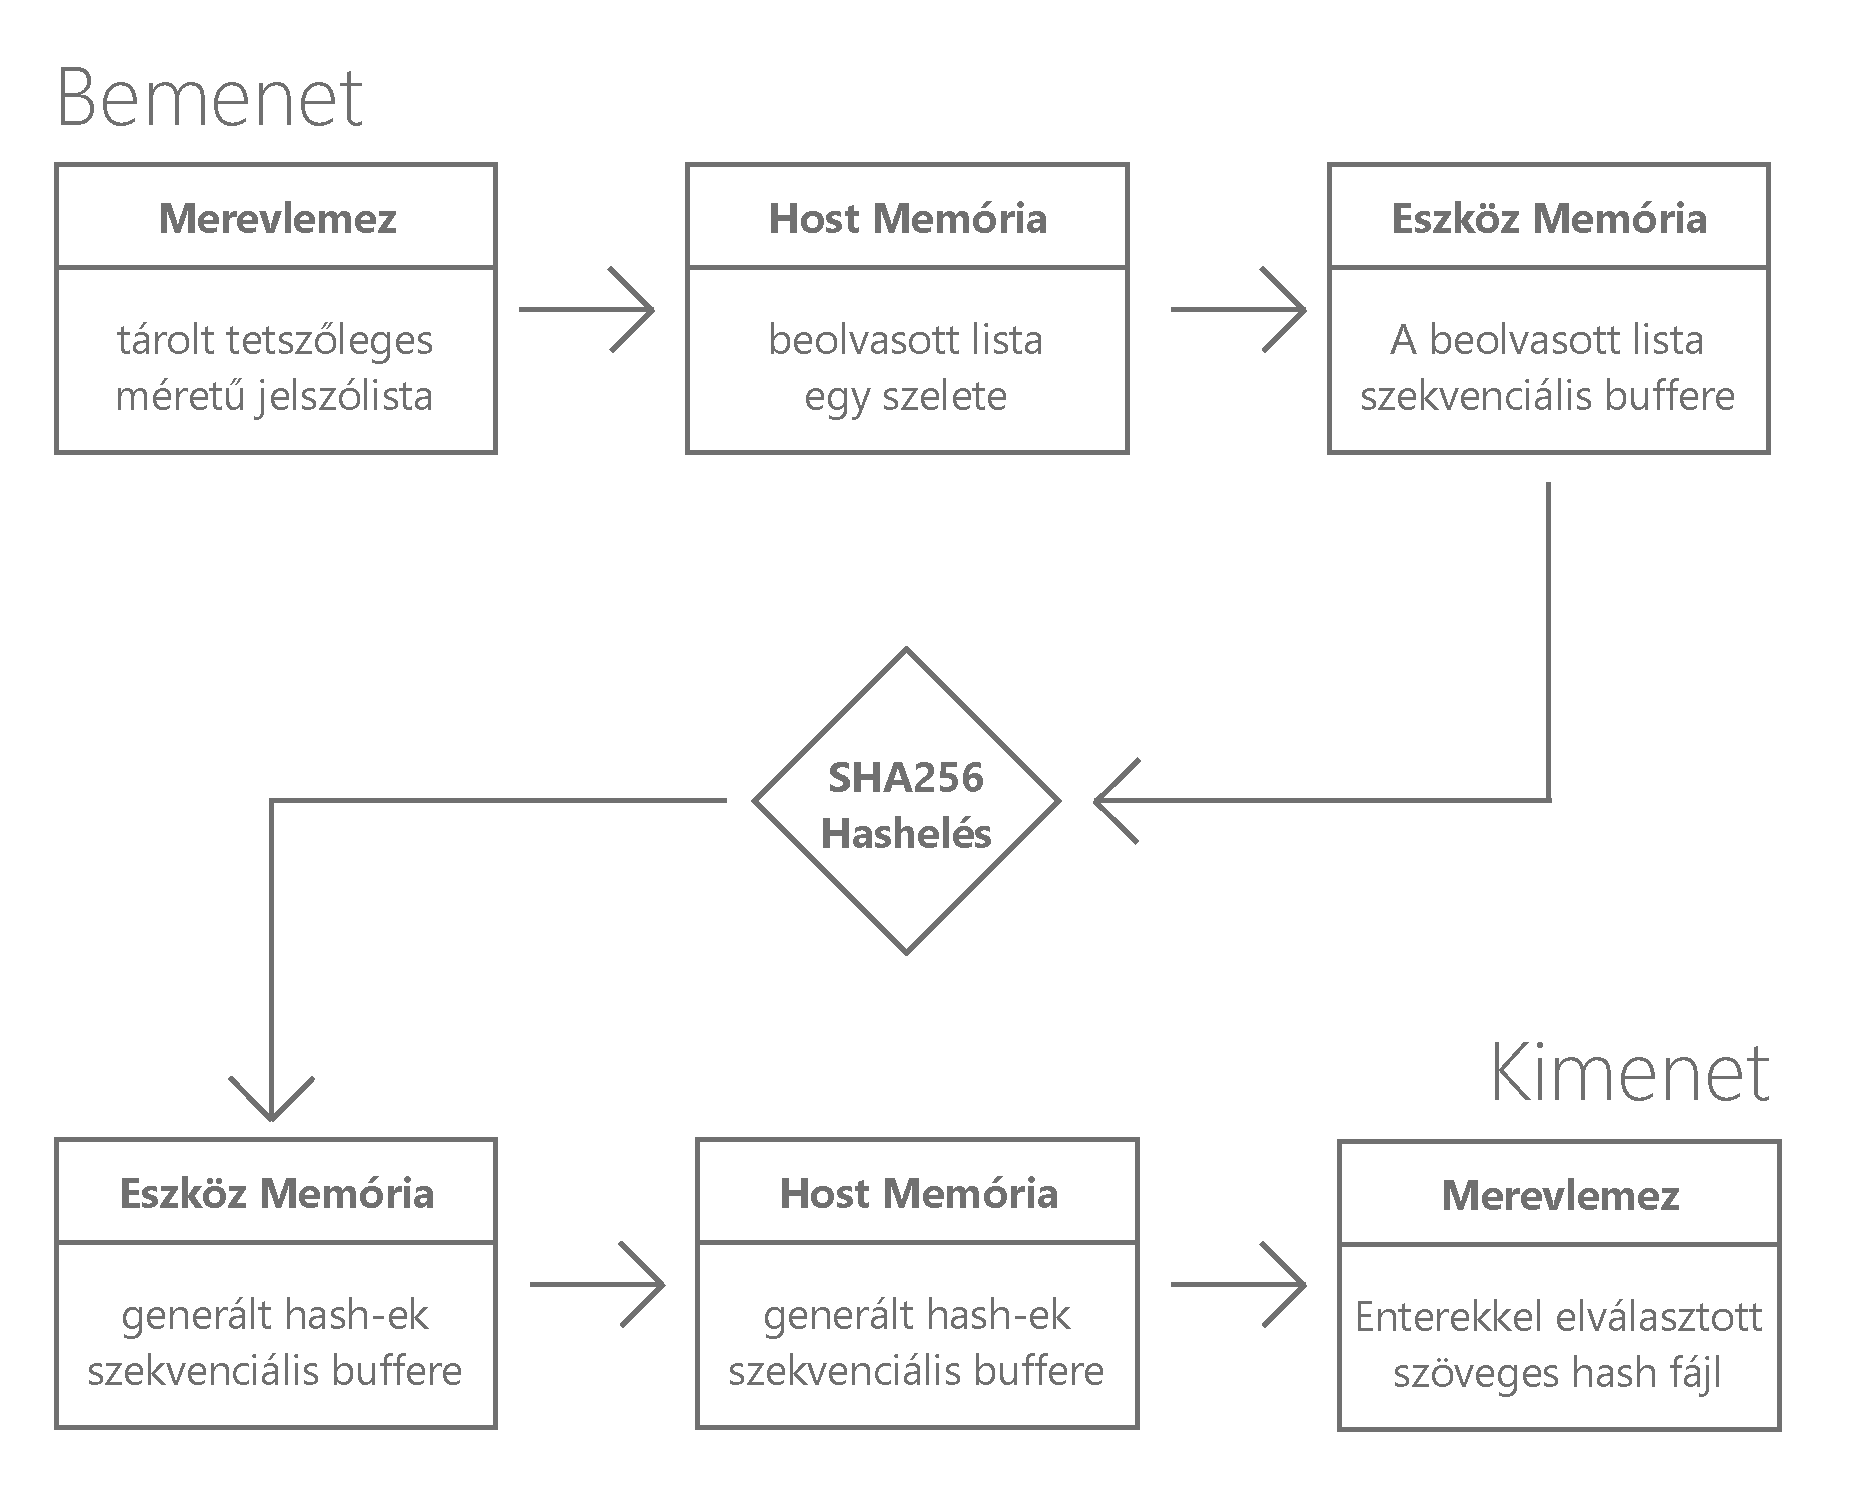
\includegraphics[width=\textwidth]{images/pdf/data-movement.pdf}
    \caption{Adatmozgazás egy fájl tartalmának hashelése során.}
    \label{fig:lineargpu}
\end{figure}


Az ábrából látható, hogy amennyiben a hashelés közben történő adatmozgatást nem vesszük figyelembe, összesen 5 különböző alkalommal kell majd másolnunk. Ezen adatmásolások közül a legtöbbet az adatok beolvasása illetve kiírása fogja igényelni. A második leglassabb a host és az eszköz memória közötti mozgatás, így aztán ezeket próbálom a lehető legjobban parallelizálni. Ahogy befejeződött a merevlemezről történő beolvasás és az továbbításra került az eszköz felé, egyből kezdhetjük a következő adatbeolvasást a merevlemezről.


\begin{figure}[H]
    \centering 
    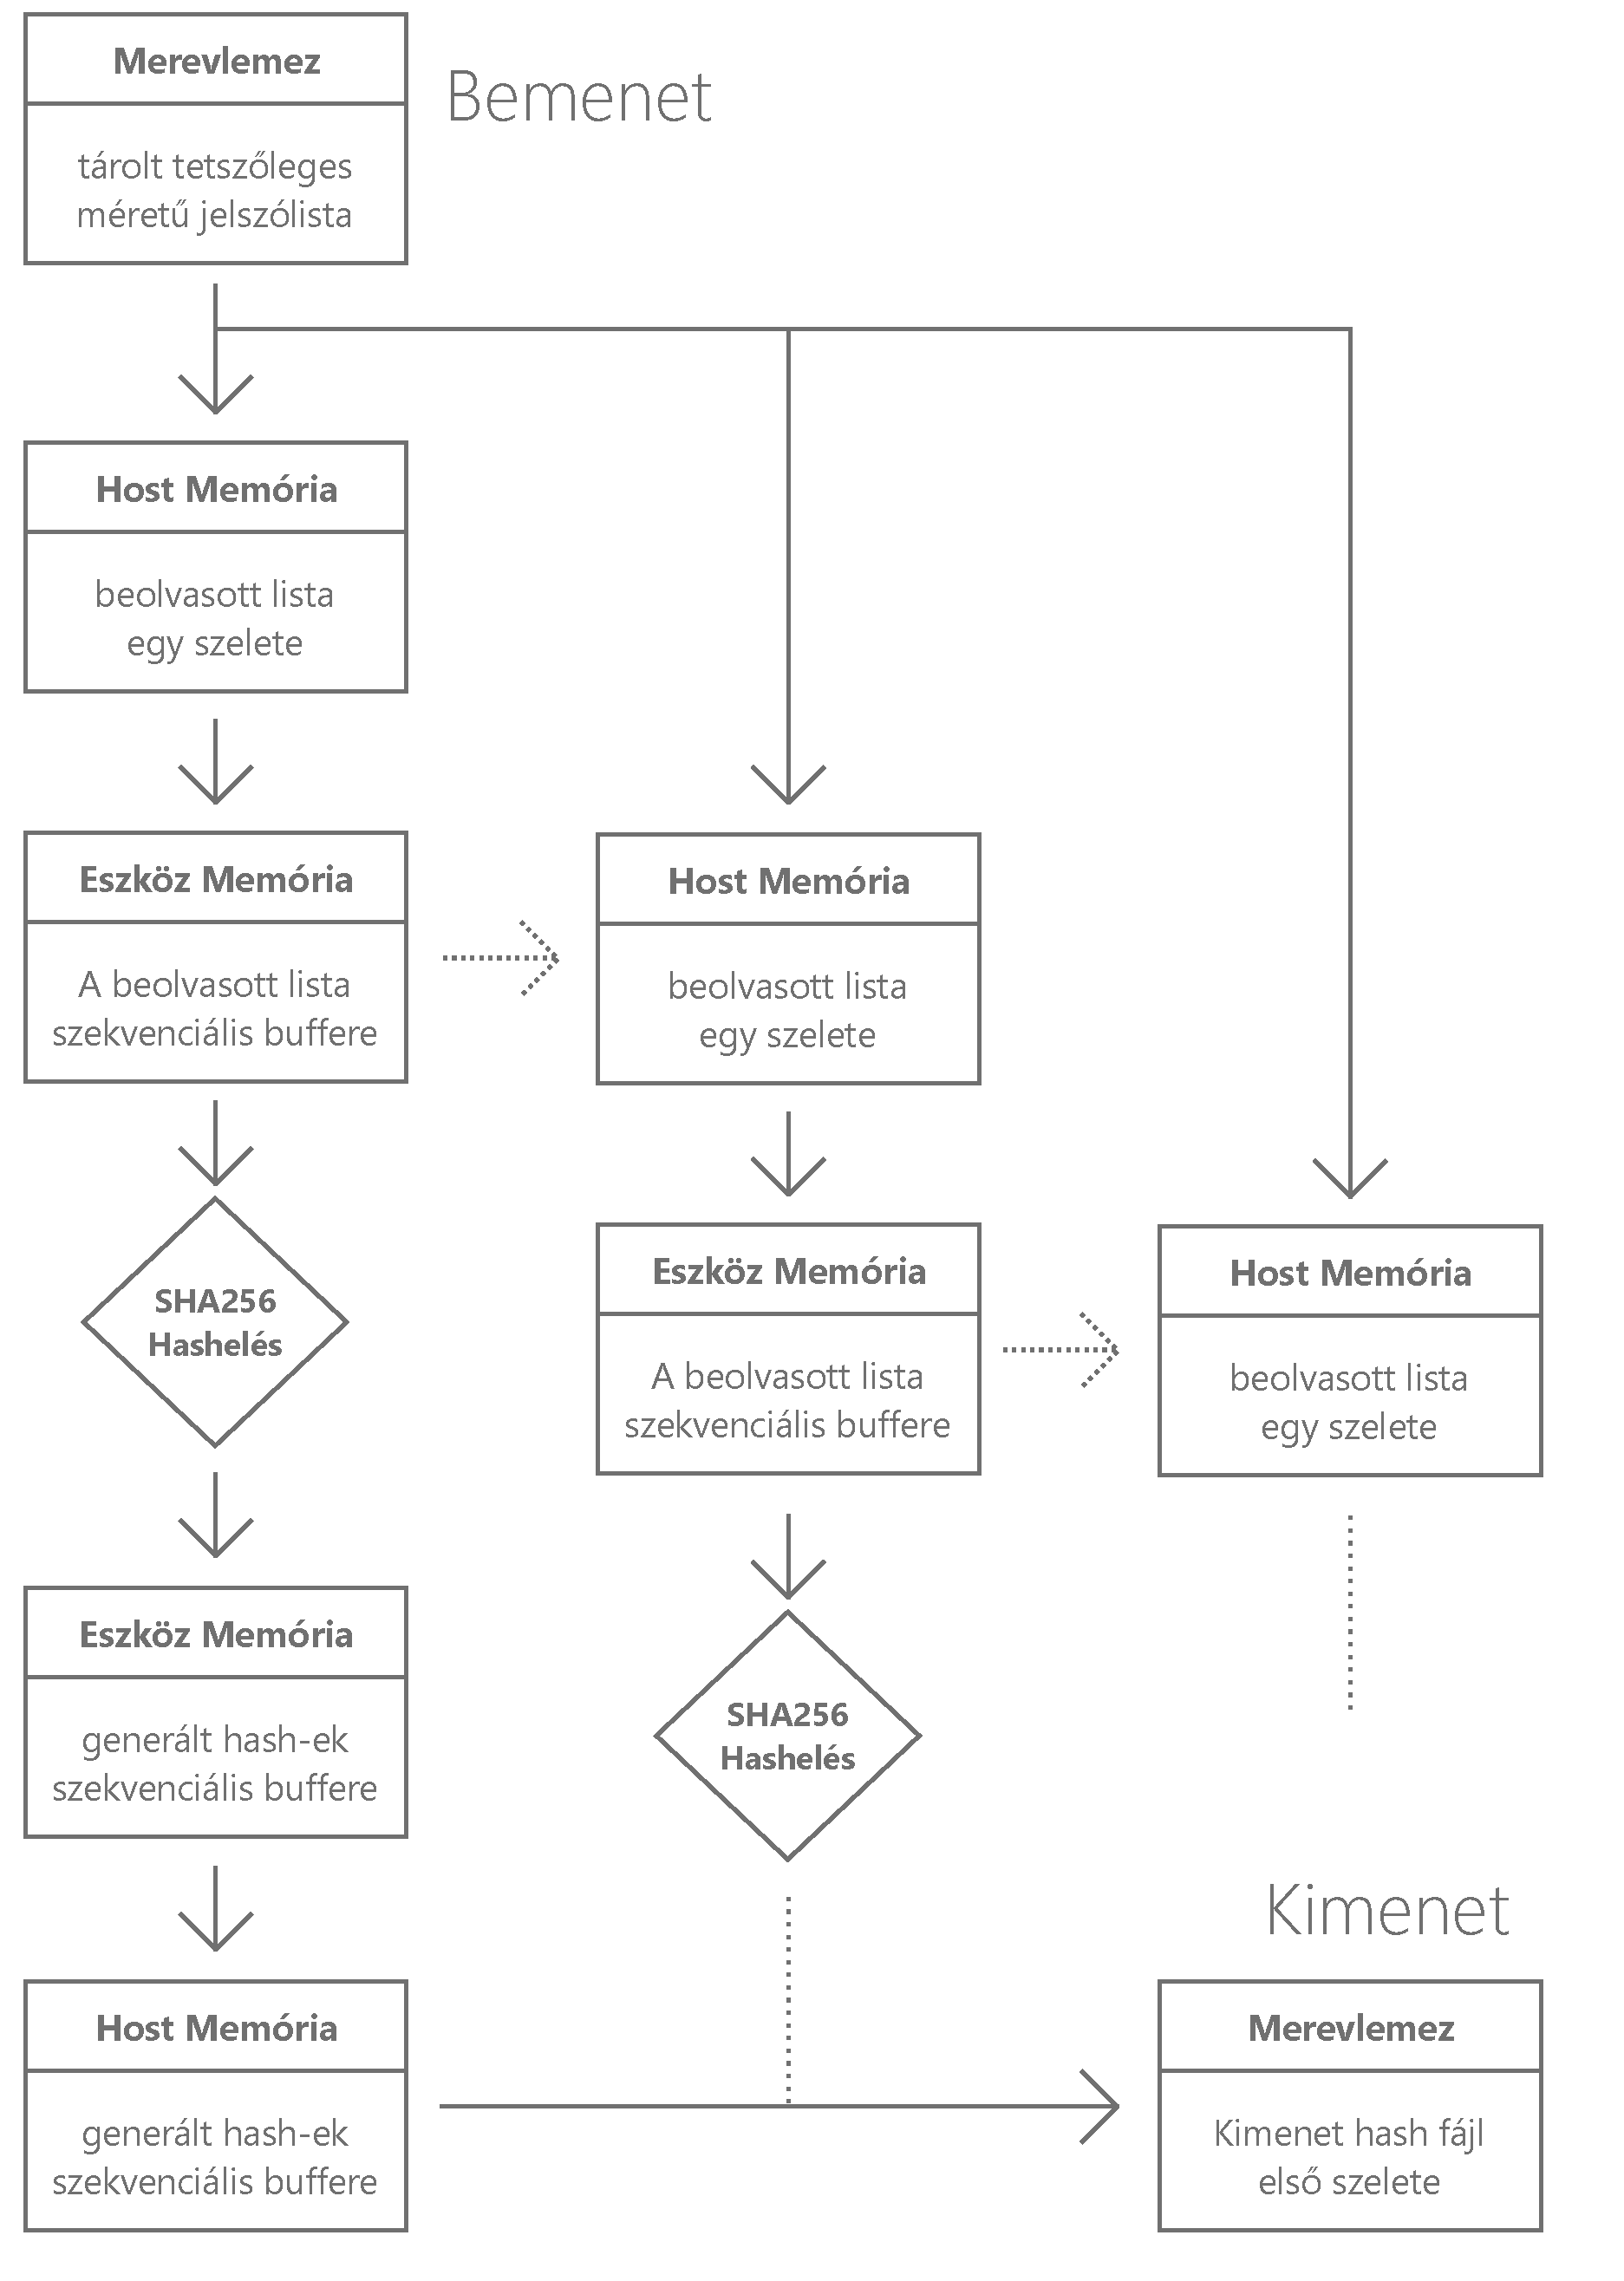
\includegraphics[width=\textwidth]{images/pdf/data-movement-parallel.pdf}
    \caption{Adatmozgazás parallel módon egy fájl tartalmának hashelése során.}
    \label{fig:parallelgpu}
\end{figure}



% Data
\subsection{Hashelés}

Az SHA256 algoritmus lépései egy hashen belül nem párhuzamosíthatóak. Az algoritmus így lett elkészítve, hiszen ha parallelizálható lenne akkor könnyebben feltörhető lennei, hiszen:
%
\begin{itemize}
    \item Egy hashelés részei gyorsíthatóak lennének, hiszen egy egy hashen sok szál tudna dolgozni egyszerre, ezzel exponenciálisan gyorsítva a feltörést,
    \item egy hashelés részekre bontható lenne, azaz bizonyos jelszavak részeinek kiszámolásához nem lenne szükség mindig előről újraszámolni részeket, hiszen azt egyszer már kiszámoltuk.
\end{itemize}
%
Több jelszó hashelése azonban nem függ egymástól, így az egyszerre futtatható feltörések számának kizárólag az eszköz és a beolvasás sebessége szab határt. A jelszavak parallel feltöréséhez szükség van egy fix méretű bemeneti és kimeneti bufferre, amelyen belül a szálak ki tudják számolni a pontos bemeneti és kimeneti pontjukat a következőképp:

Legyen:
\begin{itemize}
    \itemsep-0.5em
    \item $N$ : kulcsok száma
    \item $M$ : egy kulcs maximális mérete
    \item $P_0$ : bemeneti buffer kezdőpontja, mérete: $[N * M]$
    \item $P_1$ : kimeneti buffer kezdőpontja, mérete: $[N * 65]$
    \item $I : [0 .. N-1]$ jelenlegi szál indexe
\end{itemize}


ekkor a jelenlegi szál:


\begin{itemize}
    \itemsep-0.5em
    \item Bemenetének kezdete $ = P_0 + (I * M) $
    \item Bemenetének vége $ = P_0 + (I * M) + (M - 1) $
    \item Kimenetének kezdete $ = P_1 + (I * 65) $
    \item Kimenetének vége $ = P_1 + (I * 65) + 64 $
\end{itemize}

A kimeneti hash mérete 64 karakter, melyhez hozzájön egy null vagy enter.


\begin{figure}[H]
    \centering
    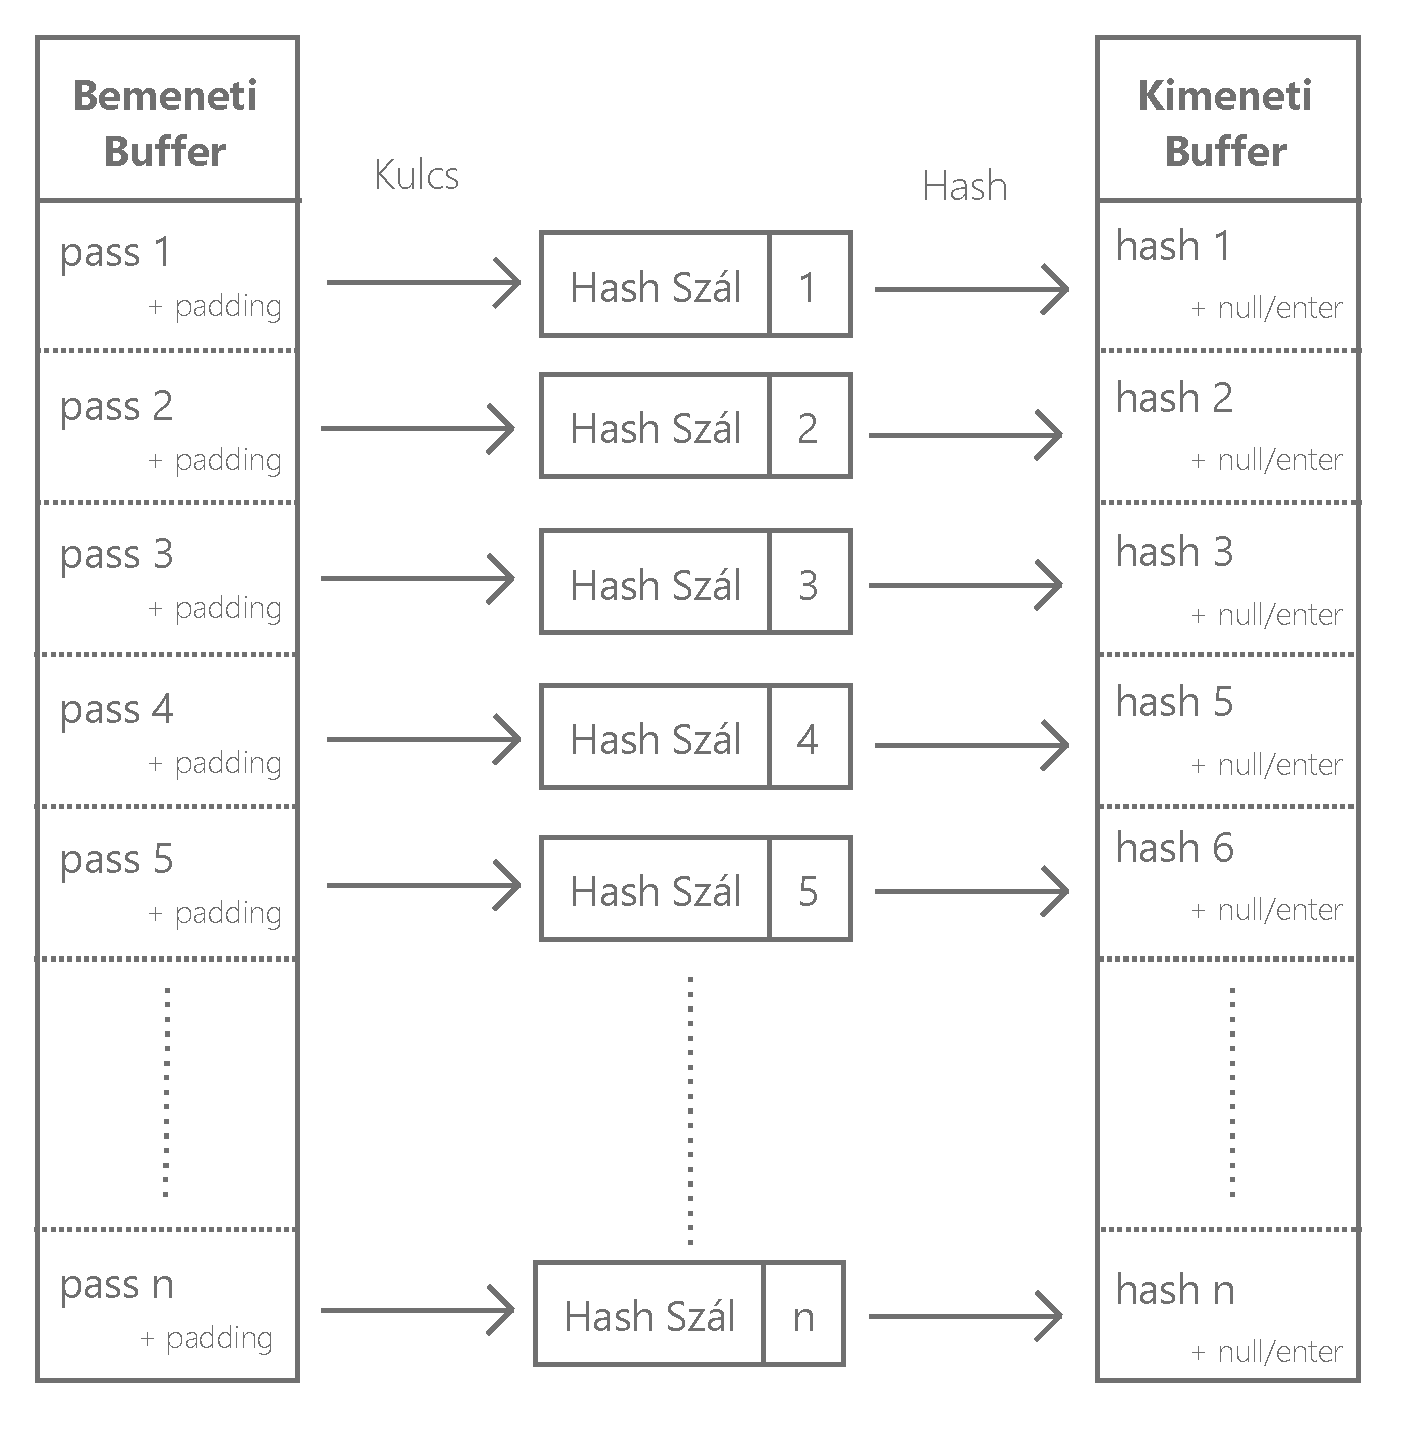
\includegraphics[width=\textwidth]{images/pdf/parallel-hashing.pdf}
    \caption{Szálak párhuzamosan dolgoznak a bemeneti kulcs bufferen és a kimeneti hash bufferen.}
\end{figure}




% Crack
\subsection{Feltörés}

Feltörés esetén azonban hashelni minden kulcsot, majd a kimenetüket kimásolni és a host-on végigiterálni egyezést keresve egy lassú és felesleges művelet lenne. Ezért ebben az esetben az első beolvasás előtt már bemásoljuk az eszköz kerneljébe a keresendő hash kódot és salt-ot és kizárólag egyezés esetén várunk választ az output bufferbe.

Legyen:
\begin{itemize}
    \itemsep-0.5em
    \item $ N $ : kulcsok száma
    \item $ M $ : egy kulcs maximális mérete
    \item $ S $ : a salt mérete
    \item $ P_0 $ : bemeneti buffer kezdőpontja, mérete: $[N * (M + S)]$
    \item $ P_1 $ : kimeneti buffer kezdőpontja, mérete egy 4 byte-os egész számnak felel meg
    \item $ I : [0 .. N-1]$ jelenlegi szál indexe
\end{itemize}


ekkor a jelenlegi szál:


\begin{itemize}
    \itemsep-0.5em
    \item Bemenetének kezdete $ = P_0 + (I * M) + (I * S) $
    \item Bemenetének vége $ = P_0 + (I * M) + (I * S) + (M + S - 1) $
    \item Kimenete $ = P_1 $, vagy nincs kimenet
\end{itemize}

Alapértelmezetten a kimenet bufferének értéke 0-ról indul. Ha a kimenet a futás után is nulla marad, akkor nem találtunk egyező kulcsot. Ezzel szemben amennyiben az érték megváltozott, akkor tudjuk hogy az adott azonosítójú szál oldotta meg sikeresen a visszafejtést és az értéket ki tudjuk olvasni az előbb betöltött memóriaterületről.


\begin{figure}[H]
    \centering
    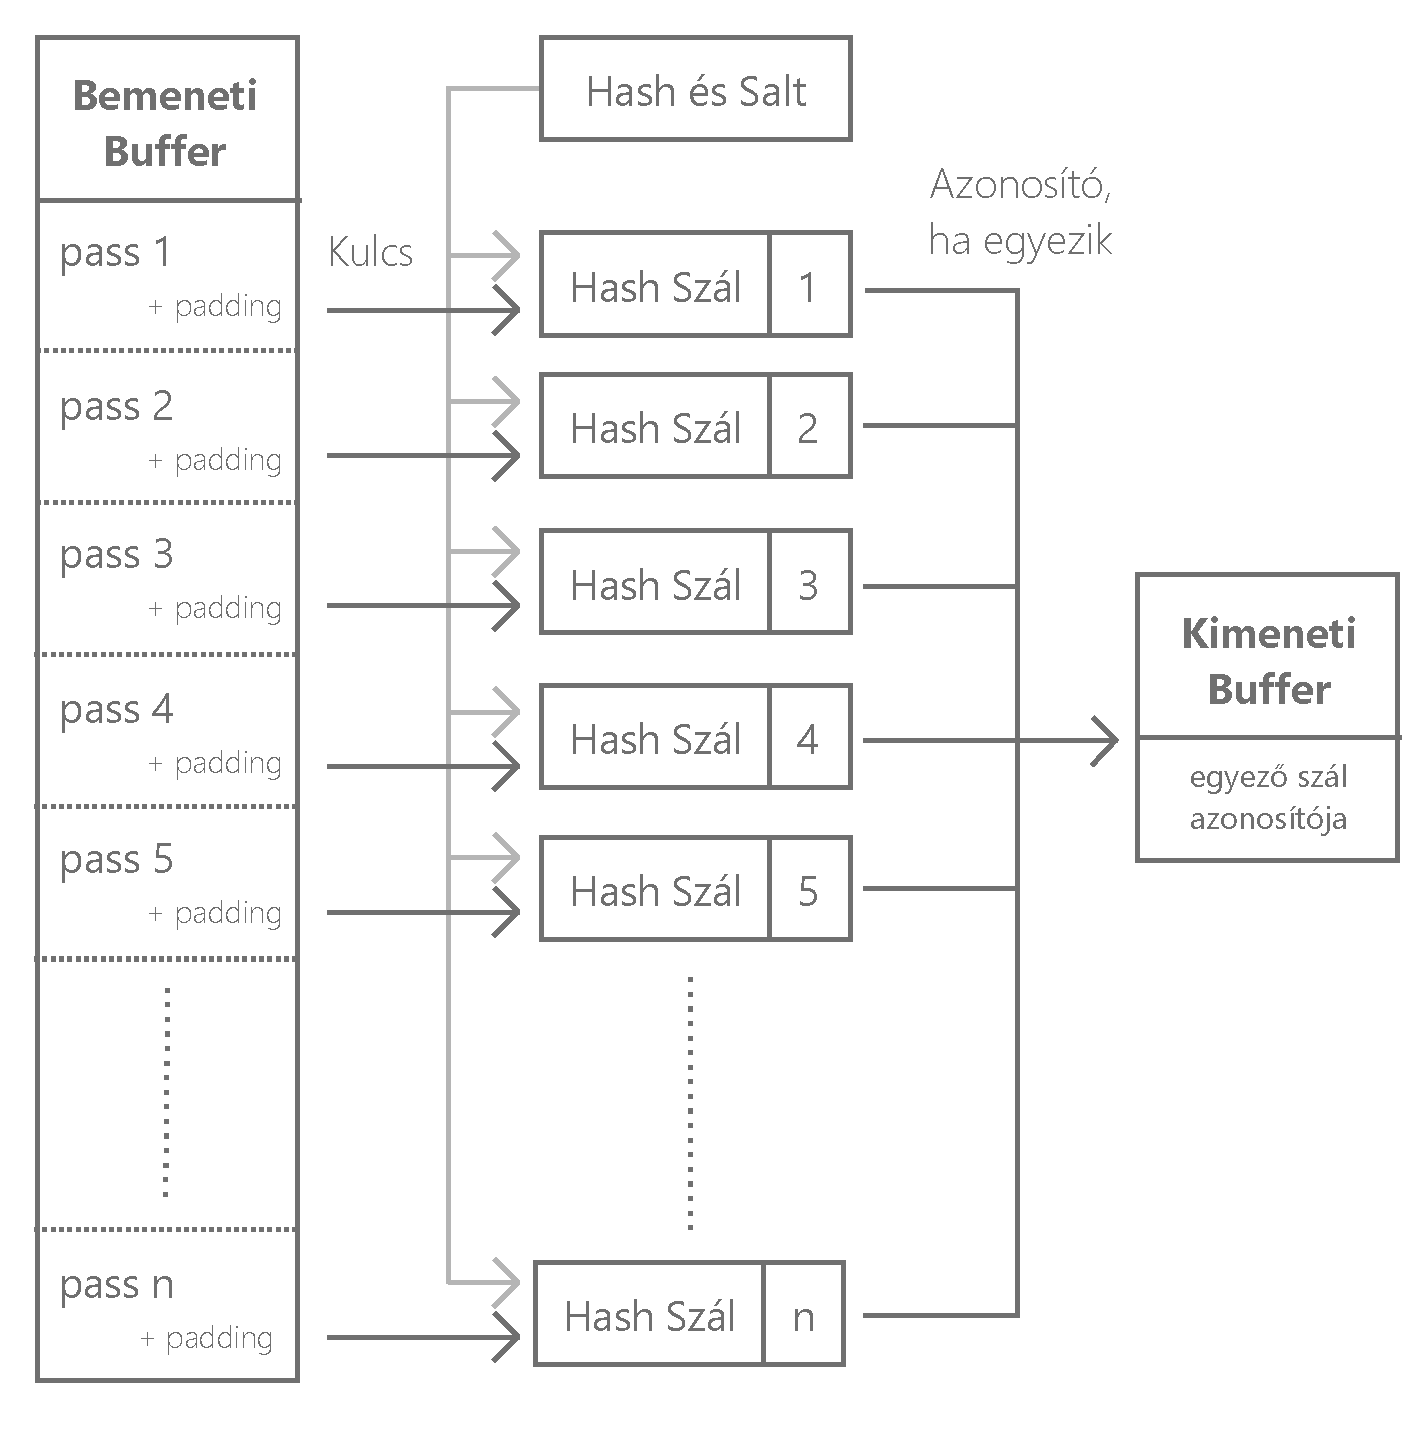
\includegraphics[width=\textwidth]{images/pdf/parallel-cracking.pdf}
    \caption{Szálak párhuzamosan dolgoznak a bemeneti kulcs bufferen és a megadott hash és salt értékeken.}
\end{figure}










% ------------------- Optimization
\section{C++ Optimalizálás}


A fejlesztési idő jelentős részét az optimalizálás töltötte ki. Miután volt egy programom, amely képes volt jelszavakat beolvasni és feltörni processzoron és videókártyán is egyből tudtam tesztelni a sebességet. A teszteléshez minden alkalommal egy 4 millió (\num{3735367}) elemű listát használt a program, melynek az utolsó elemeként szerepelt a helyes kulcs (ex-wethouder).
A futási idő méréséhez a C++ nyelv standard környezetében található chrono könyvtárat használtam, amely képes microsec pontossággal jelezni két utasítás között eltelt időt. Az végleges időkben kizárólag a tényleges feltöréssel töltött idő szerepel, nem tartalmazza az elején az inicializálsát és a fájl megnyitását, illetve a végén az eredmény kiiratását. Ezek ugyanis egyszer történnek csak meg, és tetszőlegesen nagy adattömeg esetén elenyésző a hatásuk.
A program debug mód kikapcsolásával és x64 architektúrára van építve, illeve a /O2 fordító paranccsal, amely többek között a kódoptimalizálást a futtatható fájl mérete helyett a sebességre fókuszálja.


\begin{definition}
Futási Stabilitás: Egy program futás időtartamának relatív eltérése több teszten keresztül azonos paraméterekkel, azonos hardveren és azonos alap kihasználtsággal.
\end{definition}

\begin{definition}
Hash per Second (h/s): Egy mértékegység amely egy algoritmus egy másodperc alatt elkészíthető hash kódjainak számára, egy adott hash algoritmus használatával, azonos hardveren és azonos alap kihasználtsággal.
\end{definition}




% First sim
\subsection{Első Szimuláció}


Az alap tesztet 20 alkalommal futtattam CPU és GPU használatával is. Ezáltal egyrészt tisztán láthatjuk az egymáshoz képest számolt sebességkülönbséget, másrészt amennyiben a függvény futási ideje instabil, korrigálhatunk arra.


\begin{table}[H]
    \centering
    \begin{tabular}{l|l|l|l}
        \textbf{Eszköz} & \textbf{Salt} & \textbf{Futásidő} & \textbf{Teljesítmény}  \\
        \hline
        \hline
        \multirow{2}{*}{CPU} & Nem & $\num{105 658 927} \; \mu s \approx \num{106.7}s$ & $\approx \num{35 353} \; h/s$ \\
                             \cline{2-4}
                             & Igen & $\num{116 019 598} \; \mu s \approx \num{116.0}s$ & $\approx \num{32 196} \; h/s$ \\
                             \hline
                             
        \multirow{2}{*}{GPU} & Nem & $\num{21 250 652} \; \mu s \approx \num{21.3}s$ & $\approx \num{175 776} \; h/s$ \\
                             \cline{2-4}
                             & Igen & $\num{21 490 658} \; \mu s \approx \num{21.5}s$ & $\approx \num{173 814} \; h/s$ \\
    \end{tabular}
    \caption{?}
\end{table}


%amcharts.com
\begin{figure}[H]
    \centering
    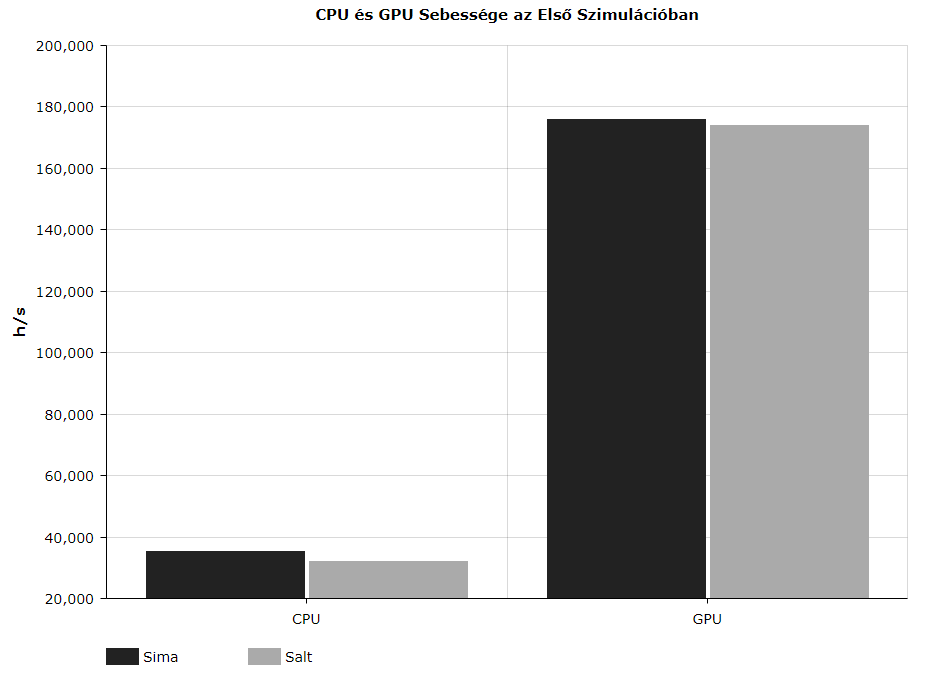
\includegraphics[width=\textwidth]{images/charts/performance-1.png}
    \caption{CPU és GPU simán és salt-al történő összehasonlítása az első szimuláció során.}
\end{figure}

Látható a szimulációs eremdményekből, hogy a GPU feltörés sebessége jelenleg a CPU megfelelőjének majdnem 550\%-a. Továbbá megfigyelhető az is, hogy a hash alkalmazása nagyobb teljesítmény veszteséget okoz CPU-nál esetén (10\%), mint GPU esetén 1\%. Ez minden bizonnyal annak tudható be, hogy az utóbbinál a videókártyán történik a salt behelyezése a szöveg végére, így ez egy időben akár ezerszer is lefuthat.

A GPU-n salt használatával történő feltörés a projekt célja, ezért erre fókuszáltam futási stabilitás tesztelésénél. A teszt során 20 alkalommal futtattam a programot azonos körülmények között.



\begin{table}[H]
    \centering
    \begin{tabular}{rl}
        \begin{tabular}{r|l}
            \textbf{Iteráció} & \textbf{Futásidő} \\
            \hline
            \hline
            1.  & $\num{21 490 792} \mu s$ \\
            2.  & $\num{21 490 518} \mu s$ \\
            3.  & $\num{21 490 488} \mu s$ \\
            4.  & $\num{21 490 178} \mu s$ \\
            5.  & $\num{21 490 213} \mu s$ \\
            6.  & $\num{21 490 968} \mu s$ \\
            7.  & $\num{21 490 446} \mu s$ \\
            8.  & $\num{21 490 978} \mu s$ \\
            9.  & $\num{21 490 792} \mu s$ \\
            10. & $\num{21 490 534} \mu s$ \\
        \end{tabular}
        
        & 
        
        \begin{tabular}{r|l}
            \textbf{Iteráció} & \textbf{Futásidő} \\
            \hline
            \hline
            11. & $\num{21 490 768} \mu s$ \\
            12. & $\num{21 490 999} \mu s$ \\
            13. & $\num{21 490 703} \mu s$ \\
            14. & $\num{21 490 744} \mu s$ \\
            15. & $\num{21 490 776} \mu s$ \\
            16. & $\num{21 490 688} \mu s$ \\
            17. & $\num{21 490 688} \mu s$ \\
            18. & $\num{21 490 702} \mu s$ \\
            19. & $\num{21 490 182} \mu s$ \\
            20. & $\num{21 490 518} \mu s$ \\
        \end{tabular}\\
    \end{tabular}
    \caption{Futási Stabilitás vizsgálatánál a tesztek futási eredményei}
\end{table}


\begin{figure}[H]
    \centering
    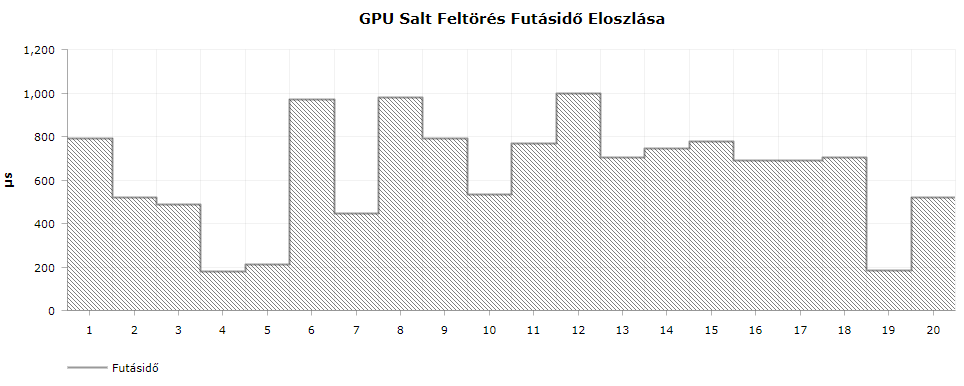
\includegraphics[width=\textwidth]{images/charts/performance-1-distribution.png}
    \caption{GPU Salt Feltörés Futásidő Eloszlása milliomod másodpercben számolva.}
\end{figure}


Ebből kiszámolható hogy az adatok szórása (standard deviation) $\sigma = 240\mu s$. Ilyen kis számoknál a programnyelv belső órájának pontossága is közrejátszhat az inkonzisztenciában, ezért a szórás a hibakorlátunk alatt helyezkedik el, tehát kijelenthetjük hogy a jelenlegi algoritmus futásideje stabil.



% Double Buffer
\subsection{Double Buffer}



Jelenleg az adatok beolvasása az \ref{fig:lineargpu} ábrának megfelelően zajlik, tehát megtörténik egy adatszegmens beolvasása, amely továbbításra kerül a feltörésre használt eszköz számára majd az eredmény megérkezését követően elkezdődik a következő beolvasás. Ezen természetesen tudunk javítani a  \ref{fig:parallelgpu} ábrának megfelelően. Erre egy dupla bufferezéses megoldást alkalmaztam, amely esetén a beolvasott adatoknak két egyforma méretű buffer lett létrehozva. Ezek legyenek $B_1, B_2, B_c, B_o \; (current, other)$
%
\begin{enumerate}
    \itemsep-0.5em
    \item $ B_c := B_1, B_o := B_2 $
    \item $ read(B_c) $
    \item $ crack(B_c) $ \& $ read(B_o) $
    \item $ swap(B_c, B_o) $
    \item back to 3.
\end{enumerate}

A bufferek méretének kiválasztását nem lehet fordításnál eldönteni, hiszen attól függnek, hogy a feltörésre használt rendszer adatok olvasása vagy az eszköz sebessége a kisebb keresztmetszet. Ezért a bufferek méretének megválasztásást a felhasználóra bízzuk, azomban a program mindenképpen választ magának egy alapértelmezett értéket, amennyiben egyéb utasítást nem kap. 

\begin{table}[H]
    \centering
    \begin{tabular}{l|l|l|r|l}
        \textbf{Lépés} & \textbf{Futásidő} & \textbf{Teljesítmény} & \textbf{Különbség} & \textbf{Javítás} \\
        \hline
        \hline
        
        CPU & $\num{116 019 598} \; \mu s \approx \num{116.0}s $ & $\approx \num{32 196} \; h/s$ & & \\
        \hline
                            
        GPU & $\num{21 490 658} \; \mu s \approx \num{21.5}s $ & $\approx \num{173 814} \; h/s$ & $+550.2\%$ & \\
        \hline
        
        GPU & $\num{20 201 236} \; \mu s \approx \num{20.2}s $ & $\approx \num{173 814} \; h/s$ & $+9.5\%$ & Double Buffer \\
        \hline
    \end{tabular}
    \caption{Teljesítmény táblázat salt-al és a double buffer hozzáadásával.}
\end{table}





% Preprocessor const
\subsection{Preprocesszor Konstansok}

A kulcs maximális mérete, a hash numerikus felbontása, a salt és annak a hossza már ismertek a kernel fordítása során és konstans értékek maradnak a teljes feltörés folyamata alatt. A just-in-time fordításnak köszönhetően ezeket az érékeket beleépíthetjük a kódba preprocesszor direktívák segítségével, ezáltal segítve a fordítót az optimalizálásban és kevesebb adatmozgatás és buffer létrehozással. Ezeket az értékeket a fordítónak adjuk át plusz paraméterként.

\begin{lstlisting}[language={C++}]
-D DEFINED_STRING=somestring
\end{lstlisting}

Egy kisebb kihívást a szöveg beszúrása jelentette a salt esetén, ugyanis a preprocesszor nem támogatja ezt. Ezt egy makro használatával tudtam megoldani.

\lstset{caption={Macro a fordítási paraméterként megkapott szöveg konvertálására.}, label=src:cpp}
\begin{lstlisting}[language={C++}]
//String convert macro
#define STR(s) #s
#define XSTR(s) STR(s)

//...

const char* str = XSTR(DEFINED_STRING);
\end{lstlisting}

Ez a konvertálás természetesen nem fog lassítani a futáson, hiszen megtörténik fordításnál.


\begin{table}[H]
    \centering
    \begin{tabular}{l|l|l|r|l}
        \textbf{Lépés} & \textbf{Futásidő} & \textbf{Teljesítmény} & \textbf{Különbség} & \textbf{Javítás} \\
        \hline
        \hline
        
        CPU & $\num{116 019 598} \; \mu s \approx \num{116.0}s $ & $\approx \num{32 196} \; h/s$ & & \\
        \hline
                            
        GPU & $\num{21 490 658} \; \mu s \approx \num{21.5}s $ & $\approx \num{173 814} \; h/s$ & $+550.2\%$ & \\
        \hline
        
        GPU & $\num{20 201 236} \; \mu s \approx \num{20.2}s $ & $\approx \num{173 814} \; h/s$ & $+9.5\%$ & Double Buffer \\
        \hline
        
        GPU & $\num{20 112 915} \; \mu s \approx \num{20.1}s $ & $\approx \num{174 509} \; h/s$ & $+0.4\%$ & Preprocessor \\
        \hline
        
        GPU & $\num{3 034 589} \; \mu s \approx \num{3.0}s $ & $\approx \num{1 157 085} \; h/s$ & $+665.7\%$ & C std IO \\
        \hline
    \end{tabular}
    \caption{Teljesítmény táblázat salt-al és a double buffer hozzáadásával.}
\end{table}



% C IO
\subsection{C Bemenet}



Jelenleg a C++ eszközeit használom a fájl beolvasására. Ez a módszer std::string struktúrába másolja a fájl sorait, ahonnan később ki kell csomagolni és beleírni a bufferbe C alapú (null karakterrel lezárt) char* -ként.


\lstset{caption={Fájl sorainak beolvasása C++ fstream eszközökkel.}, label=src:cpp}
\begin{lstlisting}[language={C++}]
std::ifstream infile(fileName);

// ...

std::string line;
for (int i = 0; i < chunkSize && std::getline(infile, line); i++)
{
    strcpy(&currentBuffer[MAX_KEY_SIZE * i], line.c_str());
}

// ...

infile.close();
\end{lstlisting}


A példán az adatfolyan egy szegmensének beolvasása található. Ez a kód (5-9. sor) ismétlődik egészen addig, amíg elfogy a fájl, vagy az előző beolvasás feltörése sikeresen zárul. Látható hogy a beolvasás során a nyelv az adatokat egy std::fstream objektumon keresztül olvassa be, amelyet egy std::string-ben helyez el. Ezt a string-et végül egy null karakterrel terminált C string-re konvertáljuk és belemásoljuk a buffer megfelelő szegmensébe. Érezhető, hogy ezek felesleges extra műveletek, amelyek a futási idő egy jelentős részét jelenthetik.

Az optimalizáláshoz leváltottam a C++ nyelv által használt iostream és fstream eszközöket a standard C könyvtárra (stdio.h).

\lstset{caption={Fájl sorainak beolvasása C++ fstream eszközökkel.}, label=src:cpp}
\begin{lstlisting}[language={C}]
FILE* infile = fopen(fileName, "r");

// ...

for (int i = 0;
     i < chunkSize && fgets(&currentBuffer[MAX_KEY_SIZE * i], MAX_KEY_SIZE, infile) != NULL;
     i++)
     { }

// ...

fclose(infile);
\end{lstlisting}


Ebben az esetben látszik, hogy a fájlből történő beolvasás azonnal a bufferbe helyezi a szöveget. Egy hátrány, hogy a szövegek nincsenek lezárva null karakterekkel, hanem a sor beolvasója behelyezi a sorok végén található sortörés karaktert. Ezt minden szövegnél ki kell javítani hogy ne tekintse a hash algoritmus az entert is a jelszó részének (hiszen azok nem tartalmazhatjak sortörés karaktert). Ezt azonban a crack-et végző eszköz végzi, így módosítottam hogy a hashelés előtt az eszköz ellenőrzi a szöveg pontos hosszát úgy, hogy null vagy enter karakterig iterál, majd a végére fűzi a salt-ot.


\lstset{caption={Fájl sorainak beolvasása C++ fstream eszközökkel.}, label=src:cpp}
\begin{lstlisting}[language={C++}]
//Get key
uint length;
globalID = get_global_id(0);
globalKey = keys + globalID * KEY_LENGTH; //Get pointer to key
for (length = 0; length < KEY_LENGTH && (globalKey[length] != '\0' && globalKey[length] != '\n'); length++)
{
    key[length] = globalKey[length];
}

//Append salt
#pragma unroll
for (uint i = 0; i < SALT_LENGTH; i++)
{
    key[length + i] = XSTR(SALT_STRING)[i];
}
length += SALT_LENGTH;
key[length] = 0;
\end{lstlisting}


Látható, hogy a kulcs lokális memóriába történő másolása során a jelenlegi karakter hozzáadása előtt megnézzük, hogy a karakter null ($\setminus 0$), vagy sortörés-e. ($\setminus n$). Amennyiben igen, a kulcs végére értünk és a length értéket nem növeljük tovább.

\begin{table}[H]
    \centering
    \begin{tabular}{l|l|l|r|l}
        \textbf{Lépés} & \textbf{Futásidő} & \textbf{Teljesítmény} & \textbf{Különbség} & \textbf{Javítás} \\
        \hline
        \hline
        
        CPU 1 & $\num{116 019 598} \; \mu s \approx \num{116.0}s $ & $\approx \num{32 196} \; h/s$ & & \\
        \hline
                            
        GPU 1 & $\num{21 490 658} \; \mu s \approx \num{21.5}s $ & $\approx \num{173 814} \; h/s$ & $+550.2\%$ & \\
        \hline
        
        GPU 2 & $\num{20 201 236} \; \mu s \approx \num{20.2}s $ & $\approx \num{173 814} \; h/s$ & $+9.5\%$ & Double Buffer \\
        \hline
        
        GPU 3 & $\num{20 112 915} \; \mu s \approx \num{20.1}s $ & $\approx \num{174 509} \; h/s$ & $+0.4\%$ & Preprocessor \\
        \hline
        
        GPU 4 & $\num{3 034 589} \; \mu s \approx \num{3.0}s $ & $\approx \num{1 157 085} \; h/s$ & $+665.7\%$ & Cstdio \\
        \hline
    \end{tabular}
    \caption{Teljesítmény táblázat salt-al és a double buffer hozzáadásával.}
\end{table}



\begin{figure}[H]
    \centering
    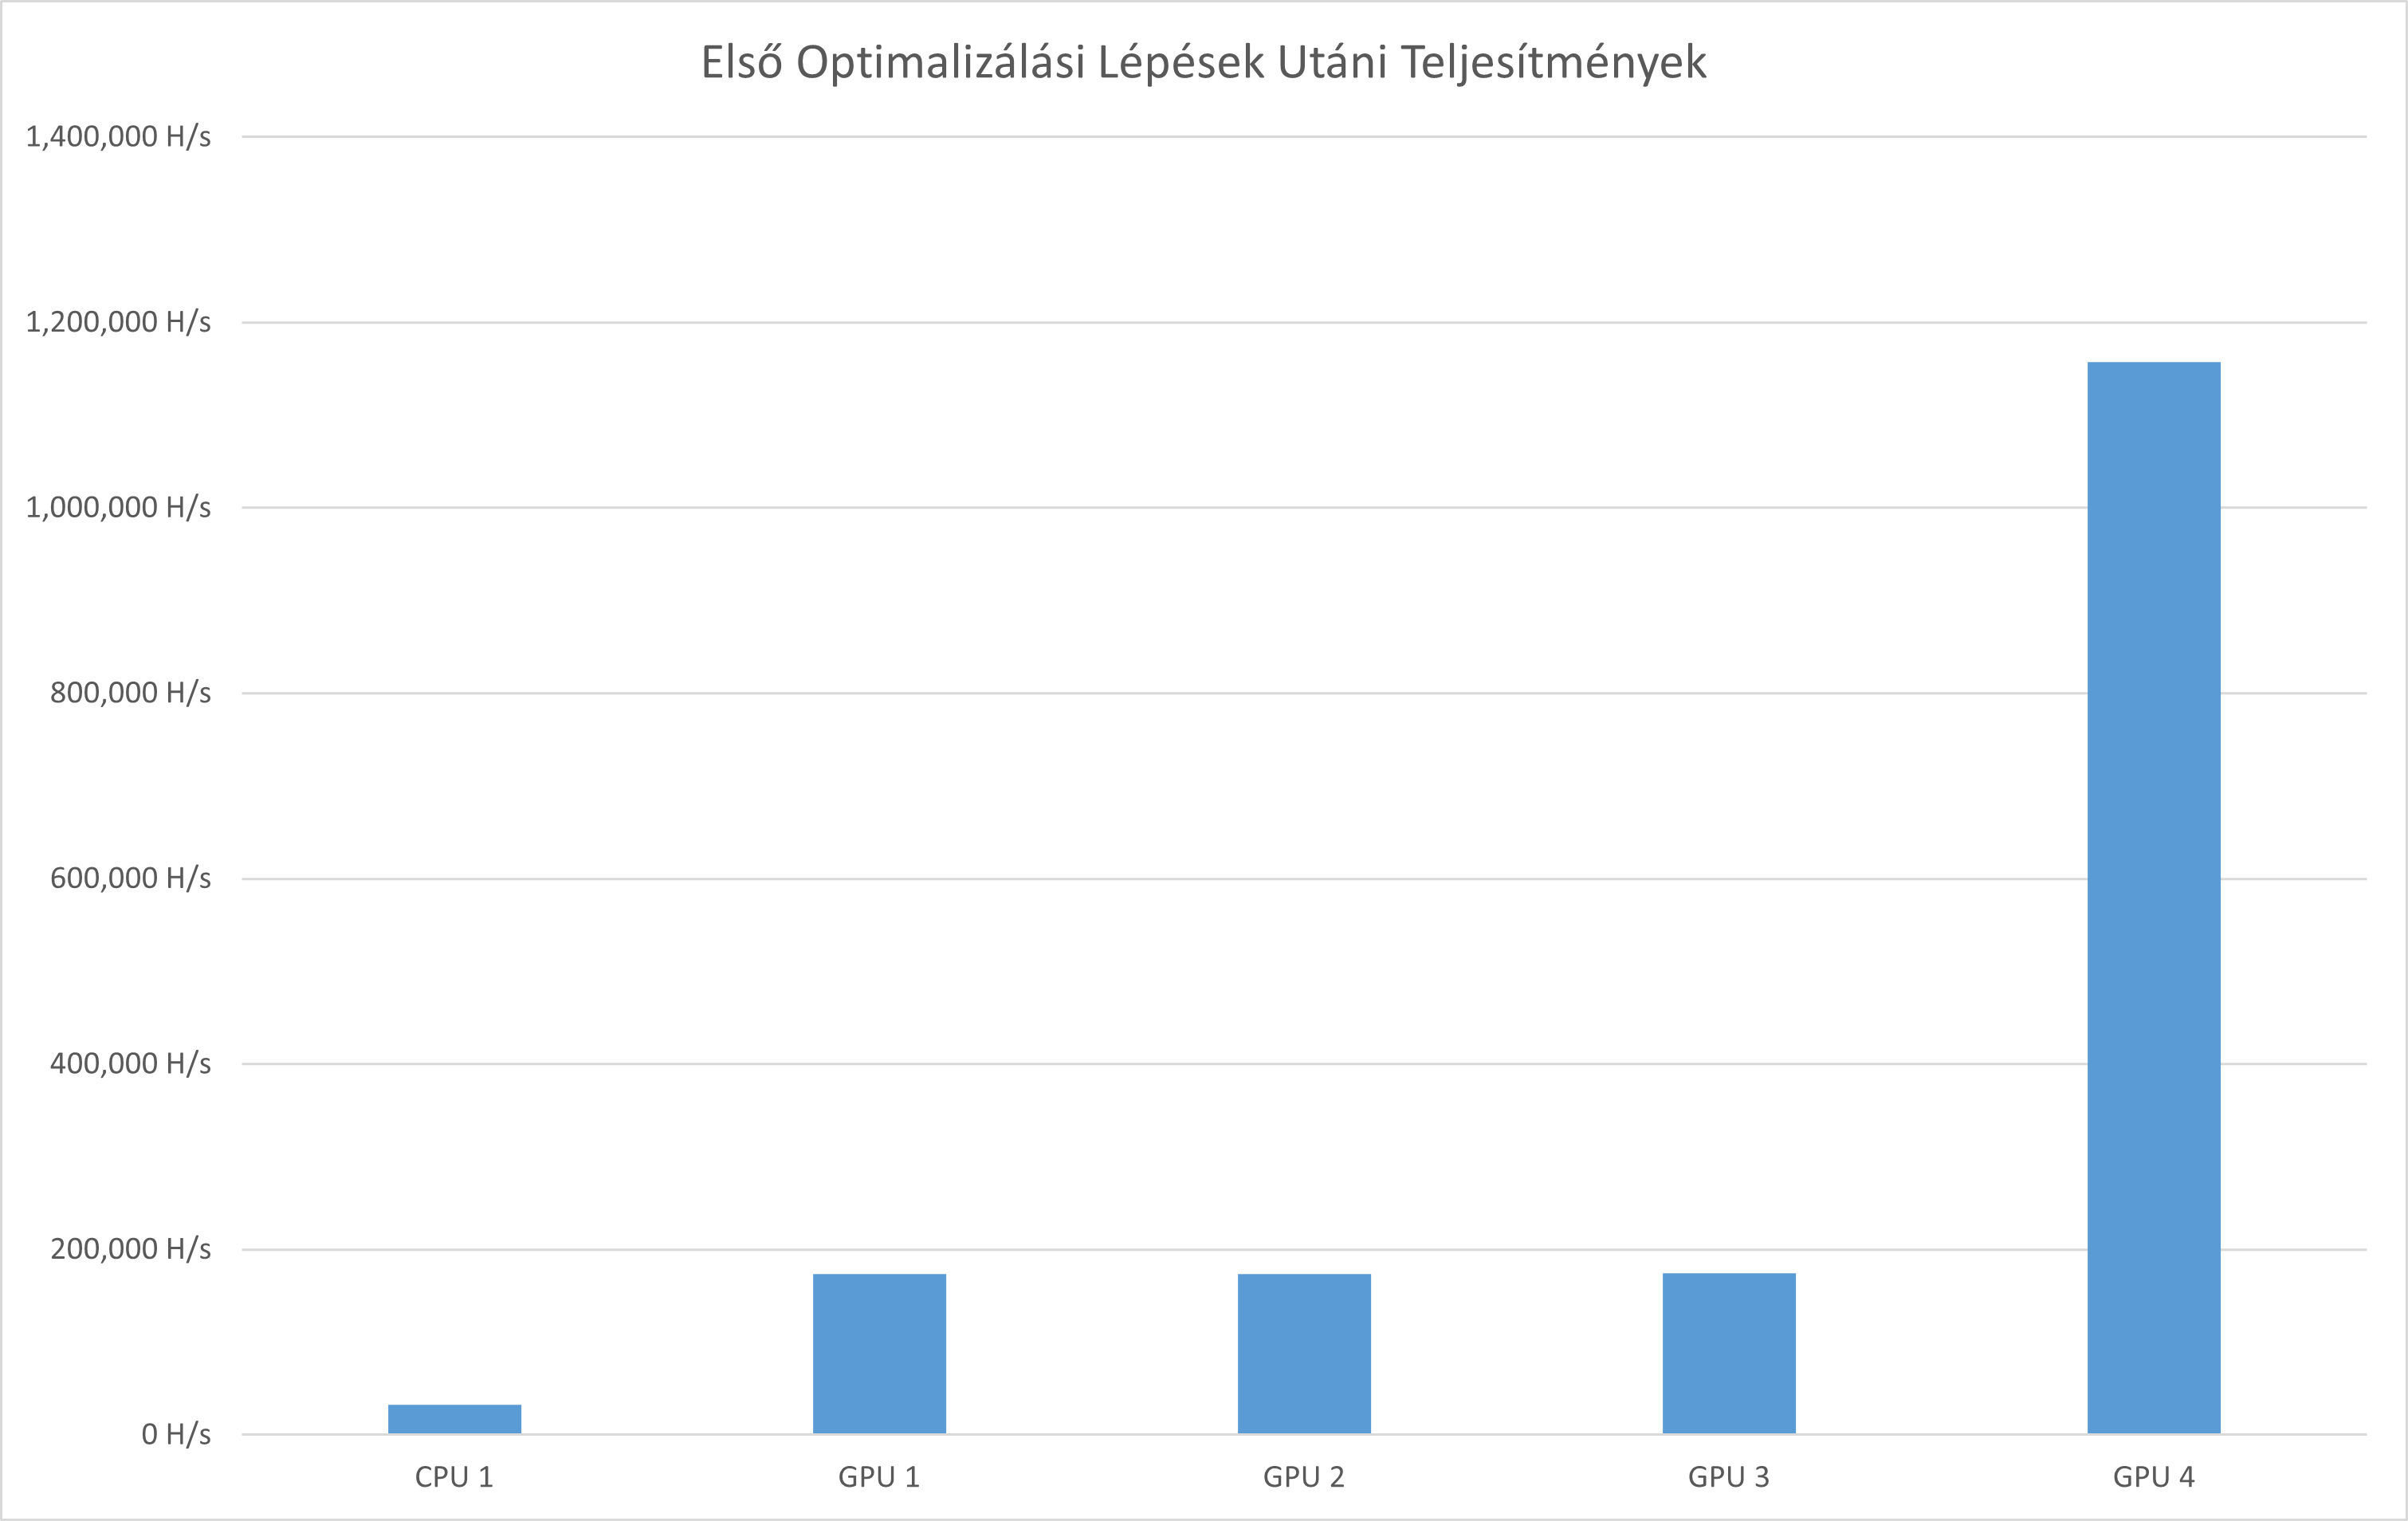
\includegraphics[width=\textwidth]{images/charts/performance-1-optimization.png}
    \caption{Az első optimalizálási lépések utáni teljesítmények összehasonlítása.}
\end{figure}





% Compiler settings x64 release
\subsection{Fordító Beállítások}

Eddig minden teszt x86 rendszerre lett fordítva Debug módban alap optimalizálási beállításokkal MSVC-ben. Ezen lehet javítani első sorban Release módra való átállással és egyéb fordító beállításokkal amelyek a futási sebességet szem előtt tartva végeznek módosításokat az assembly-n. Ehhez átalakítottam a függőségi fát a GPGPU órán tanultakról és integráltam az OpenCL fájlokat a projektbe. Ez önmagában nem működőképes, mert az OpenCL headerek bizonyos deklarációi kizárólag Debug fordítás esetén voltak elérhetőek. Ezeket a limitációkat eltávolítottam ezen műveletek inline metódusokká alakításával.

Ezek mellett le kellett töltenem az OpenCL előre fordított könyvtárának x64-es verzióját, amelyre a fordító és a linker megfelelő konfigurálásával sikerült átállítani a rendszert. A módok között a Visual Studio program-ban a fordítási beállításoknál lehet váltani.

\begin{figure}[H]
    \centering
    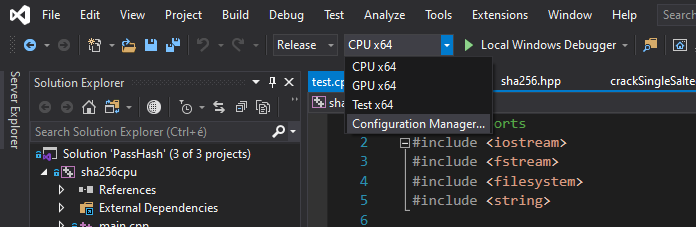
\includegraphics[width=\textwidth]{images/illustrations/visualstudio-compile-modes.png}
    \caption{A fordítási mód kiválasztása a Visual Studio-ban.}
\end{figure}

A megfelelő build módot kiválasztva a főmenüben található "Build" $\xrightarrow{}$ "Build Solution" kombninációval indíthatjuk, amely kizárólag a meghatározott programot építi majd fel a Solution-ből.

Az architektúra választó mezőtől közvetlenül balra találjuk a fordítási mód beállítóját. Debug módban továbbra is bekerülnek az MSVC által definiált debug környezeti segítő metódusok és hook-ok. Ezzel szemben a release verziónál a fordító a maximális optimalizálás érdekében a következő paranccsal fordul:

\lstset{caption={A Release mód fordításának parancsa MSVC használatával.}, label=src:cpp}
\begin{lstlisting}[language={bash}]
MSVC_COMPILER_PATH\bin\HostX86\x64\CL.exe /c /I..\oclpack\include\ /Zi /nologo /W3 /WX- /diagnostics:column /sdl /O2 /Ob2 /Oi /Ot /GT /GL /D WIN64 /D NDEBUG /D _CONSOLE /D _UNICODE /D UNICODE /Gm- /EHsc /MD /GS /Gy /fp:precise /permissive- /Zc:wchar_t /Zc:forScope /Zc:inline /Fo".\build\obj\gpu-release\\" /Fd".\build\obj\gpu-release\vc142.pdb" /Gd /TP /FC /errorReport:prompt crackSingle.cpp crackSingleSalted.cpp GPUController.cpp hashMultiple.cpp platformDetails.cpp hashSingle.cpp hashSingleSalted.cpp main.cpp
\end{lstlisting}


\begin{table}[H]
    \centering
    \begin{tabular}{l|l|l|r|l}
        \textbf{Lépés} & \textbf{Futásidő} & \textbf{Teljesítmény} & \textbf{Különbség} & \textbf{Javítás} \\
        \hline
        \hline
        
        CPU 1 & $\num{116 019 598} \; \mu s \approx \num{116.0}s $ & $\approx \num{32 196} \; h/s$ & & \\
        \hline
                            
        GPU 1 & $\num{21 490 658} \; \mu s \approx \num{21.5}s $ & $\approx \num{173 814} \; h/s$ & $+550.2\%$ & \\
        \hline
        
        GPU 2 & $\num{20 201 236} \; \mu s \approx \num{20.2}s $ & $\approx \num{173 814} \; h/s$ & $+9.5\%$ & Double Buffer \\
        \hline
        
        GPU 3 & $\num{20 112 915} \; \mu s \approx \num{20.1}s $ & $\approx \num{174 509} \; h/s$ & $+0.4\%$ & Preprocessor \\
        \hline
        
        GPU 4 & $\num{3 034 589} \; \mu s \approx \num{3.0}s $ & $\approx \num{1 157 085} \; h/s$ & $+665.7\%$ & Cstdio \\
        \hline
        
        GPU 5 & $\num{1 083 921} \; \mu s \approx \num{1.0}s $ & $\approx \num{3 239 422} \; h/s$ & $+279.9\%$ & Release/x64 \\
        \hline
    \end{tabular}
    \caption{Teljesítmény táblázat salt-al és a double buffer hozzáadásával.}
\end{table}




% Thread size
\subsection{Szálméret}

Ezen az optimalizálást nem számolom bele a végleges értékekbe, ugyanis az eddigieknél is kevésbé konzisztens. Általánosan elmondható volt idáig, hogy a pontos teljesítmény nem fog megfelelni két rendszer között, azonban arányaiban megfeleltethető lesz, azaz egy kétszeres teljesítmény növelés nagyjából ugyan ekkora különbséggel jár majd minden rendszeren.
A programnak megadható a -t kapcsoló használatával, hogy hány kulcsot töltsön fel a memóriába feltörésre egy időben. Az optimális mennyiség sok faktortól függ és ami nálam jelentős terljesítmény növekedést eredményez, az egy másik rendszeren többszörös lassulást jelenthet. Ezért ahelyett hogy egy általános megoldást találnék a problémára, a felhasznlálónak meghagyom a lehetőséget hogy ő döntse el, vagy kísérletezze ki a megfelelő értéket.
Az én rendszerem esetén a megfelelő érték nagyjából $t = \num{22000}$

\begin{figure}[H]
    \centering
    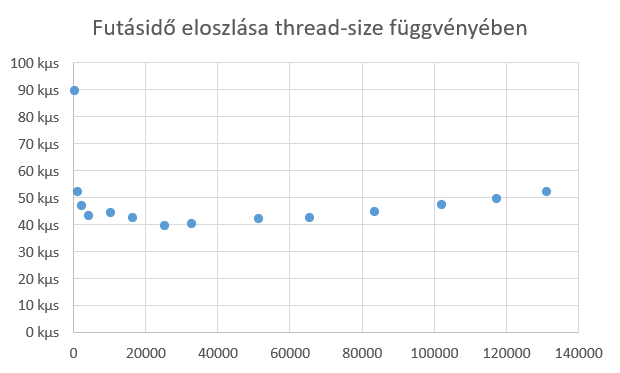
\includegraphics[width=\textwidth]{images/charts/thread-size-performance.png}
    \caption{Teljesítmény különbség szálméret arányában az én rendszeremen.}
\end{figure}

Az ábrán látható hogy $t = \num{5000}$ alatt jelentősen csökken a teljesítmény, hiszen az idő egyre nagyobb részét teszi ki a bufferek mozgatása és a kernel elindítása. A teljesítménykülönbség az én rendszeremen $t = \num{1}$ és $t = \num{22000}$ között 1102 szeres. $t = \num{22000}$ felett lassan romlik a teljesítmény.


% ------------------- opencl OCL Optimization
\section{OpenCL Optimalizálás}

Az OpenCL oldalon is hasonlóan jelentős teljesítmény növelés érhető el a feltörő algoritmus refaktorálásával. Az eredeti kódban vannak felesleges kódok, amelyek nem lesznek használva, illetve optimalizálatlan és egyszerűsíthető részek. Az egyik elsődleges szempont az elágazások eliminálása és balanszolása lesz, ugyanis ezeknél egy videókártyának minden leheőségen végig kell mennie hogy ki tudja elégíteni a lehetőségek számát minden szálra. 




% Compiler settings x64 release
\subsection{Lokális Memória}

A beérkező kulcsokat a globális memóriából kapjuk meg, ahol melléjük írjuk a salt-ot, majd onnan másoljuk át a kezdeti bufferbe. Ez azt eredményezi, hogy sok feleselges üres memória másolódik át, illetve többször a lassú globális területen dolgozunk. Erre megoldásként az eszközön létre kell hoznunk egy memóriaterületet, amely tárolja a kulcs és a hash összefűzött szöveget. A dinamikus memóriafoglalás azomban jelentősen lassítana a műveleten, ezért kihasználom azt, hogy előre ismerjük a kulcs maximális hosszát és a salt pontos méretét. Ennek köszönhetően létre lehet hozni előre minden szálon a szükséges területeket, amely minimális számítási költséggel jár. Az adatok átmásolásához végigiterál a program a kapott globális kulcson és átmásolja a karaktereket, majd mögéhelyezi a salt-ot.

\lstset{caption={A kucs lokális memóriába másolása az eszközön.}, label=src:cpp}
\begin{lstlisting}[language={C++}]
//Local memory for the key (+1 for terminating null)
char key[KEY_LENGTH + SALT_LENGTH + 1];

//Get pointer to key string
char* globalKey = keys + get_global_id(0) * KEY_LENGTH;

//Copy key
for (length = 0; length < KEY_LENGTH && (globalKey[length] != 0 && globalKey[length] != '\n'); length++)
{
    key[length] = globalKey[length];
}

//Append salt
#pragma unroll
for (uint i = 0; i < SALT_LENGTH; i++)
{
    //Get salt from preprocessor definition
    key[length + i] = XSTR(SALT_STRING)[i];
}
length += SALT_LENGTH;

//Closing null
key[length] = 0;
\end{lstlisting}

Mivel a jelszó nem tartalmazhat sortörés karaktert, ezért addig vizsgáljuk a szöveget, amíg nem találunk egyet vagy egy szövegzáró null-t.



% Compiler settings x64 release
\subsection{Kulcs Konvertálása}


A kulcsot a hasheléshez egy uint tömbbe kell konvertálnunk. Mivel minden karakter 8 bit, ezért pontosan 4 karakter fér bele egy integer-be. Így amíg néggyel egészként osztható a kulcs hossza, pontosan belefér egész mennyiségű int-be.

\lstset{caption={A kucs néggyel egészen osztható részének az uint tömbbe másolása.}, label=src:cpp}
\begin{lstlisting}[language={C++}]
//Copy whole uints
qua = length / 4;
mod = length % 4;
for (uint i = 0; i < qua; i++)
{
    W[i]  = (key[i * 4 + 0]) << 24;
    W[i] |= (key[i * 4 + 1]) << 16;
    W[i] |= (key[i * 4 + 2]) << 8;
    W[i] |= (key[i * 4 + 3]);
}
\end{lstlisting}

Külön kell kezelni azomban amikor a kulcs hossza nem osztható n-el hiszen akkor az utolsó uint utolsó karaktere mögé egy 1-es bitet kell helyezni.

Erre egy gyors megoldást biztosít a biteltolás és a négy esetre bontás. Legyen: $K_l$ a kulcs hossa és $S_l$ a salt hossza. Ekkor a négy eset:

\begin{enumerate}
    \item $K_l + S_l \equiv 0 \; (mod \; 4) \iff n * 4 + 0 = K_l + S_l \; (n \geq 0)$
    \item $K_l + S_l \equiv 1 \; (mod \; 4) \iff n * 4 + 1 = K_l + S_l \; (n \geq 0)$
    \item $K_l + S_l \equiv 2 \; (mod \; 4) \iff n * 4 + 2 = K_l + S_l \; (n \geq 0)$
    \item $K_l + S_l \equiv 3 \; (mod \; 4) \iff n * 4 + 3 = K_l + S_l \; (n \geq 0)$
\end{enumerate}

Ezekben az esetekben másként kell kezelni az utolsó 0-3 karaktert. A szöveg végén egy 1-es bitet kell elhelyezni ezek mellett, amely az előző modulus alapú felbontás alapján rendre:

\begin{table}[H]
    \begin{tabular}{l|l|l}
        $\equiv$  & Bin                                              & Hex          \\
          \hline
    0 & $1000\;0000\;0000\;0000\;0000\;0000\;0000\;0000$ & $80000000$ \\
    1 & $1000\;0000\;0000\;0000\;0000\;0000$             & $800000$   \\
    2 & $1000\;0000\;0000\;0000$                         & $8000$     \\
    3 & $1000\;0000$                                     & $80$      
        
    \end{tabular}
    \caption{Az utolsó uint értékének a padding-je a mod érték alapján}
\end{table}

Ennek a kódja a következőképp néz ki optimalizálva a kernelben:

\lstset{caption={A kucs néggyel nem osztható részének az uint tömbbe másolása.}, label=src:cpp}
\begin{lstlisting}[language={C++}]
//Pad remaining uint with leading 1 bit
switch (mod)
{
    //l = n * 4 + 0
    case 0:
        W[qua] = 0x80000000;
        break;

    //l = n * 4 + 3
    case 3:
        W[qua]  = (key[qua * 4 + 0]) << 24;
        W[qua] |= (key[qua * 4 + 1]) << 16;
        W[qua] |= (key[qua * 4 + 2]) << 8;
        W[qua] |= 0x80;
        break;

    //l = n * 4 + 2
    case 2:
        W[qua]  = (key[qua * 4 + 0]) << 24;
        W[qua] |= (key[qua * 4 + 1]) << 16;
        W[qua] |= 0x8000;
        break;

    //l = n * 4 + 1
    case 1:
        W[qua]  = (key[qua * 4 + 0]) << 24;
        W[qua] |= 0x800000;
        break;
}

//Add key length
W[15] = length * 8;
\end{lstlisting}

Megfigyelhető, hogy a feldolgozás sorrendje 0, 3, 2, 1 a megmaradó nem egész vagy üres uint esetén. Ennek az oka statisztikai gyakoriságból ered. Az általam használt majdnem 4 millió elemű gyakran használt listában a következő hosszúságú jelszavak voltak a leggyakoribbak:

\begin{figure}[H]
    \centering
    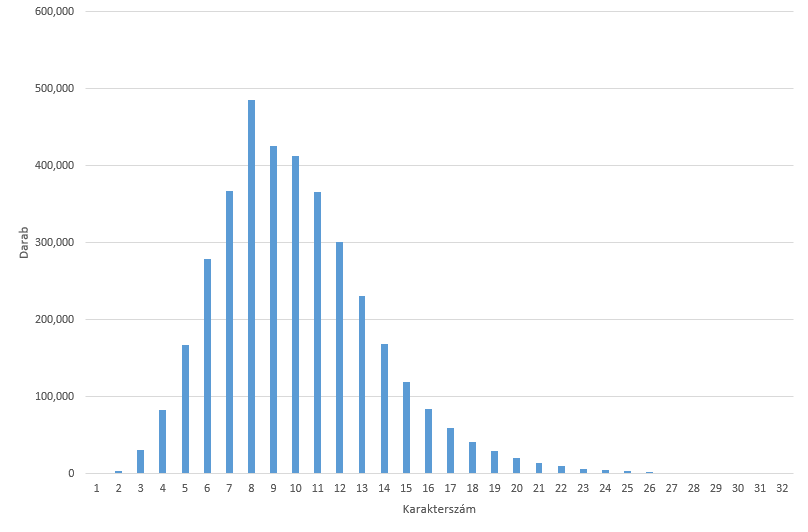
\includegraphics[width=\textwidth]{images/charts/passwords-by-length.png}
    \caption{Jelszavak hossza és gyakoriságuk majdnem 4 millió elemű listából.}
\end{figure}

\begin{figure}[H]
    \centering
    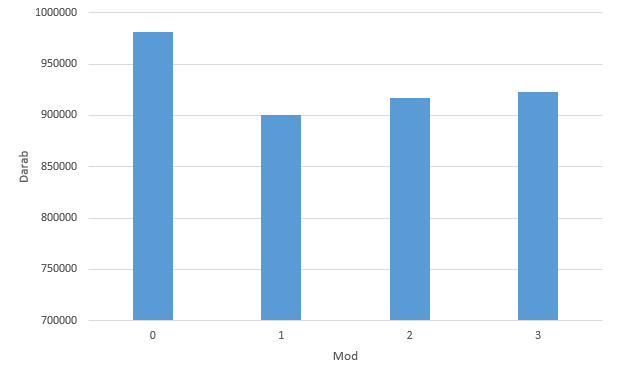
\includegraphics[width=\textwidth]{images/charts/passwords-by-length-group.png}
    \caption{Jelszavak hosszának gyakorisága mod 3-el számolva. A láthatóság kedvéért a grafikon \num{700000}-nél kezdődik.}
\end{figure}

Abban az esetben ha egy szál munkacsoportban (work group) minden elem például mod 0 és 1-re értékelődik ki, akkor nem szükséges a további két csoportot is végigszámolni. Annak érdekében hogy ez az eset a lehető leggyakrabban történjen meg, az elágazásokat a mod 4 sorrendjük alapján rendszereztem.




% Compiler settings x64 release
\subsection{Kiterjesztés és Tömörítés}


Az adatok konvertálása után a következő lépés az üzenet kiterjesztése majd tömörítése. Ezeket a legtöbb rendszerben ciklusok végzik, amelyen belül is elágazások találhatók bizonyos műveleteknek. Mivel csak egy blokkal dolgozunk, ezért ezeket statikusan is elvégezhetjük ciklusok kiterítésével. Ehhez szeparálni kell a különböző részeket és konstans hosszúságú ciklusként unroll-olni. Ennek a végeredménye egy különbontott üzenetsor

\lstset{caption={Az üzenetsor kiterjesztése a kezdeti kulcsból.}, label=src:cpp}
\begin{lstlisting}[language={C++}]
//Run message schedule
#pragma unroll
for (uint i = 16; i < 64; i++)
{
    W[i] = sig1(W[i - 2]) + W[i - 7] + sig0(W[i - 15]) + W[i - 16];
}
\end{lstlisting}


Jelen esetben a sig0(x) és sig1(x) függvények rendre a $\sigma_0(x)$ és $\sigma_1(x)$ függvényeknek felelnek meg. Az első 15 elem az üzenetet és annak hosszát tárolja, ezért a kiterjesztés 16-tól kezdődik.

Ennek a kódnak a kiemelésével a tömörírést szintén egy kiterített ciklusban tudjuk használni:

\lstset{caption={Az üzenetsor tömörítése a kezdeti kulcsból.}, label=src:cpp}
\begin{lstlisting}[language={C++}]
//Prepare compression
A = H0;
B = H1;
C = H2;
D = H3;
E = H4;
F = H5;
G = H6;
H = H7;


//Compress
#pragma unroll
for (uint i = 0; i < 64; i++)
{
    //Alter instance
    T1 = H + csig1(E) + ch(E, F, G) + K[i] + W[i];
    T2 = csig0(A) + maj(A, B, C);

    //Rotate over, override H
    H = G;
    G = F;
    F = E;
    E = D + T1;
    D = C;
    C = B;
    B = A;
    A = T1 + T2;
}
\end{lstlisting}

Látható, hogy az unroll-ok használata miatt nincsen ciklus, sem elágazás a kód ezen részében. A kiterjesztés 5. sorában található kódot például egy időben kettesével is el lehet végezni, ugyanis nem befolyásolja az $n.$ elem az $n+1$-et. Ezzel szemben az adatok forgatása miatt továbbra is egyesével kell haladnunk a második kiterjesztett ciklusban.


% Compiler settings x64 release
\subsection{Összehasonlítás}

Az összehasonlításnál alap esetben az összes hashelt blokk elemeit összegezzük, majd ezeket összehasonlítjuk. Jelenleg mivel csak egy blokk lehetséges, ezért csak az első blokk hash értékét kell hozzáadni a kiindulási értékekehez és ezt összehasonlíani az előre ismert értékekkel.

A hashelés eredménye minden esetben egy 8 elemű uint tömb lesz, amit a kiiratáshoz hexadecimális karaktersorozattá alakítunk. Jelenleg felesleges ezt átalakítani, ezért a host oldalon előre kiszámoljuk a hash uint felírását és definiáljuk azt a kernelben fordítás előtt. Ezzel egyrészt nem lesz szükséges egy nagyobb karaktertömmbe átkonvertálni az uint elemeket, másrészt az összehasonlításnál 64 byte méretű terület összehasonlítása helyett 8 darab 32 bites területet hasonlítunk.

Bontsuk a hash-et 8 részre, ahol $H$ a feltörésre szánt hash, $h$ a jelenlegi blokkból számolt hash, $D$ a kiindulási állapot és $n$ a blokkok száma. Ekkor a hash-ek egyeznek, ha minden komponensük egyezik:
%
\begin{multicols}{2}

    \begin{equation*}
        \begin{split}
            H_1 = D_1 + \sum_{i=1}^{n} h_1^i \; , \\
            H_2 = D_2 + \sum_{i=1}^{n} h_2^i \; , \\
            H_3 = D_3 + \sum_{i=1}^{n} h_3^i \; , \\
            H_4 = D_4 + \sum_{i=1}^{n} h_4^i \; , \\
        \end{split}
    \end{equation*}
    \break
    \begin{equation*}
        \begin{split}
            H_5 = D_5 + \sum_{i=1}^{n} h_5^i \; , \\
            H_6 = D_6 + \sum_{i=1}^{n} h_6^i \; , \\
            H_7 = D_7 + \sum_{i=1}^{n} h_7^i \; , \\
            H_8 = D_8 + \sum_{i=1}^{n} h_8^i \; ; \\
        \end{split}
    \end{equation*}
    
\end{multicols}

A mi esetünkben kizárólag egy blokk lesz használva, ezért az egyenletek egyszerűsíthetőek.

\begin{multicols}{2}

    \begin{equation*}
        \begin{split}
            H_1 = D_1 + h_1^1 \; , \\
            H_2 = D_2 + h_2^1 \; , \\
            H_3 = D_3 + h_3^1 \; , \\
            H_4 = D_4 + h_4^1 \; , \\
        \end{split}
    \end{equation*}
    \break
    \begin{equation*}
        \begin{split}
            H_5 = D_5 + h_5^1 \; , \\
            H_6 = D_6 + h_6^1 \; , \\
            H_7 = D_7 + h_7^1 \; , \\
            H_8 = D_8 + h_8^1 \; ; \\
        \end{split}
    \end{equation*}
    
\end{multicols}

Ezen értékekből a kernel fordításának időpontjában ismert számunkra $H$ és $D$ egy konstans érték. Ezért ezen műveletek egy részét már a fordító elvégezheti, amennyiben átrendezzük a műveleteket. Akkor bizonyítottuk hogy a megadott kulcs megegyezik a megkapott hash-el ha:
%
\begin{equation*}
    \begin{aligned}
    &h_1^1 = H_1 - D_1 \;\land\; h_2^1 = H_2 - D_2 \;\land\; h_3^1 = H_3 - D_3 \;\land\; h_4^1 = H_4 - D_4 \;\land \\
    &h_5^1 = H_5 - D_5 \;\land\; h_6^1 = H_6 - D_6 \;\land\; h_7^1 = H_7 - D_7 \;\land\; h_8^1 = H_8 - D_8;
    \end{aligned}
\end{equation*}

A programkóban a ($H_1$ ... $H_8$) $\Rightarrow$ (HASH\_0 ... HASH\_7), ($h_1$ ... $h_8$) $\Rightarrow$ (A ... H), ($D_1$ ... $D_8$) $\Rightarrow$ (H0 ... H7). Mivel az egyenlőségjelek jobb oldalán található kivonás mindkét eleme ismert fordítási időben preprocesszor definícióként, ezért a végleges kódba annak a kiszámolt verziója kerül be. Ennek köszönhetően összesen 1..8 darab egész szám egyenlőségvizsgálat fog megtörténni. Amennyiben az adott szálon bizonyítottuk a kulcsok egyezését, a szál száma plusz egy belekerül az eredmény uint-be, amelyet később a c++ oldalon kiolvasunk. A szálak számozása 0-tól indul, azonban jelenleg a 0 érték (amelyet host-tól kapunk) azt fogja jelenti, hogy nem találtuk az értéket, ezért egyezés esetén a szál számához egyet hozzá kell adnia a kernelnek.

\lstset{caption={Egyszerűsített hash egyenlőség vizsgálata.}, label=src:cpp}
\begin{lstlisting}[language={C++}]
//Verify result
if (A == HASH_0 - H0 && B == HASH_1 - H1 &&
    C == HASH_2 - H2 && D == HASH_3 - H3 &&
    E == HASH_4 - H4 && F == HASH_5 - H5 &&
    G == HASH_6 - H6 && H == HASH_7 - H7)
{
    *result = globalID + 1;
}
\end{lstlisting}

\begin{table}[H]
    \centering
    \begin{tabular}{l|l|l|r|l}
        \textbf{Lépés} & \textbf{Futásidő} & \textbf{Teljesítmény} & \textbf{Különbség} & \textbf{Javítás} \\
        \hline
        \hline
        
        CPU 1 & $\num{116 019 598} \; \mu s \approx \num{116.0}s $ & $\approx \num{32 196} \; h/s$ & & \\
        \hline
                            
        GPU 1 & $\num{21 490 658} \; \mu s \approx \num{21.5}s $ & $\approx \num{173 814} \; h/s$ & $+550.2\%$ & \\
        \hline
        
        GPU 2 & $\num{20 201 236} \; \mu s \approx \num{20.2}s $ & $\approx \num{173 814} \; h/s$ & $+9.5\%$ & Double Buffer \\
        \hline
        
        GPU 3 & $\num{20 112 915} \; \mu s \approx \num{20.1}s $ & $\approx \num{174 509} \; h/s$ & $+0.4\%$ & Preprocessor \\
        \hline
        
        GPU 4 & $\num{3 034 589} \; \mu s \approx \num{3.0}s $ & $\approx \num{1 157 085} \; h/s$ & $+665.7\%$ & Cstdio \\
        \hline
        
        GPU 5 & $\num{1 083 921} \; \mu s \approx \num{1.0}s $ & $\approx \num{3 239 422} \; h/s$ & $+279.9\%$ & Release/x64 \\
        \hline
        
        GPU 5 & $\num{308 774} \; \mu s \approx \num{0.3}s $ & $\approx \num{12 097 414} \; h/s$ & $+373.4\%$ & Kernel \\
        
    \end{tabular}
    \caption{Teljesítmény táblázat az OpenCL optimalizálások hozzáadásával.}
\end{table}

%CURRENT 3735367 compare in 0.308774 = 12 097 414 per sec